\documentclass{amsart}
\usepackage[foot]{amsaddr} % put addresses on first page

\usepackage{geometry}
\usepackage{booktabs}
\usepackage{graphicx,psfrag,epsf}
\usepackage{enumerate}
\usepackage{enumitem}
\usepackage{amsfonts}
\usepackage{mathtools}
\usepackage{amssymb}
\usepackage{amsmath}
\allowdisplaybreaks
\usepackage{longtable}
\usepackage{bigints}
\usepackage{siunitx}
\usepackage{amsthm}
\usepackage{soul}
\usepackage{color}

\usepackage{hyperref}
\usepackage[capitalise]{cleveref}
\newtheorem{theorem}{Theorem}[section]
\newtheorem{corollary}{Corollary}[theorem]
\newtheorem{lemma}[theorem]{Lemma}
%

\usepackage[numbers]{natbib}
\usepackage{url} % not crucial - just used below for the URL 
\usepackage{doi}

\title{Copula estimation using loss-based Bayesian Additive Regression Trees}
\author{**}
\date{\today}

\begin{document}

\maketitle

\section{Introduction}

\section{Model}

\subsection{Conditional copula}

Let $Y_1$ and $Y_2$ be two continuous random variables and $X$ be a continuous random variable 
that might affect the relationship between $Y_1$ and $Y_2$. 
Then according to Sklar’s theorem there exists a unique copula such that:
\begin{equation}
    H_{X}(y_1,y_2\mid x; \theta, \alpha_1, \alpha_2) = C\{F_{Y_1\mid X}(y_1\mid x;\alpha_1),F_{Y_2\mid X}(y_2\mid x; \alpha_2)\mid x;\theta\}; \quad \forall (y_1,y_2) \in \mathbb{R}^2.
\end{equation}
This gives us the following
\begin{equation}
    h_{X}(y_1,y_2\mid x; \theta, \alpha_1, \alpha_2) = f_{Y_1\mid X}(y_1\mid x;\alpha_1)f_{Y_2\mid X}(y_2\mid x; \alpha_2)c(u_1,u_2\mid x;\theta),
\end{equation}
where
\begin{equation}\label{eq:emp_dist:Y}
    u_k = F_{Y_k\mid X}(y_k\mid x; \alpha_k)
\end{equation}
and $c(u_1,u_2\mid x;\theta)$ is conditional copula density function.

\subsection{Loss-based BART}

Let $T$ denote a tree and $M$ denote the vector of terminal node values $M = \{\mu_1,\mu_2, \cdots, \mu_{n_L}\}$. Let $\theta_i$ denote the copula parameter conditional on $x_i$. Our aim is to estimate this copula parameter using a regression tree such that
\begin{equation}
	\theta_i = g(x_i, T, M)
\end{equation}
where $g$ denotes the assign rule of the tree $T$. Recently, 
a loss-based prior for regression tree is proposed by \citet{serafini2024lossbasedpriortreetopologies} in the following way:
\begin{align}
	T, M &\sim \pi(T)\pi(M\mid T)\\
	T &\propto \exp\left(\omega n_L(T)-\gamma\Delta(T)\right)\\
	\pi(M\mid T) & = \prod_{j=1}^{n_L}\pi(\mu_j\mid T).
\end{align}

\subsection{Complete hierarchical model}
As mentioned earlier, we wish to estimate the copula parameter using a regression tree. Given a set of observations $(u_{11}, u_{21}), (u_{12}, u_{22}), \cdots, (u_{1n}, u_{2n})$

\begin{align}
    u_{1i}, u_{2i} \mid \theta_i &\sim c(u_{1i},u_{2i}\mid x_i;\theta_i) \qquad i = 1,2,\cdots, n  \\
    \theta_i & = g(x_i, T, M)\\
    T, M &\sim \pi(T)\pi(M\mid T)\\
	T &\propto \exp\left(\omega n_L(T)-\gamma\Delta(T)\right)
\end{align}

For the choice of prior on $\mu_j\mid T$ a conjugate prior is suggested by \citet{chipman_BART,serafini2024lossbasedpriortreetopologies}. However, finding a conjugate prior for the copula parameter is not trivial. Instead, we use a flat-prior on the support of the copula parameter and employ Metropolis-Hastings algorithm for obtaining posterior estimates. Choice of priors are detailed in the next section for specific simulation analyses.


\iffalse

\subsubsection{Choice for $\mu_j$}
\begin{itemize}
    \item Jeffrey's prior \url{https://www2.stat.duke.edu/~berger/papers/bivariate.pdf}
    \item Simple uniform distribution in $(-1,1)$ 
    \item Transformed beta \url{https://academic.oup.com/jrsssa/article/145/2/237/7105492}
    \item Log-normal on $-\log(1-p^2)$
    \item Inverse-Gamma on $-\log(1-p^2)$
\end{itemize}
Note that for the first three choices, we only work with transformed beta distribution by 
selecting suitable hyper-parameters.

\subsection{Density of $\rho$}

Let $\kappa = -\log(1-p^2)$, then for $\rho \ge 0$
\begin{align}
	\rho & = \sqrt{1-\exp(-\kappa)}\coloneqq g(\kappa)
\end{align}

Now, let $0\le\kappa_1 < \kappa_2<\infty$, then

\begin{align}
	&g(\kappa_2) - g(\kappa_1)\\
	&=\sqrt{1-\exp(-\kappa_2)} - \sqrt{1-\exp(-\kappa_1)}\\
	&= \frac{(\sqrt{1-\exp(-\kappa_2)} - \sqrt{1-\exp(-\kappa_1)})(\sqrt{1-\exp(-\kappa_2)} + \sqrt{1-\exp(-\kappa_1)})}{(\sqrt{1-\exp(-\kappa_2)} + \sqrt{1-\exp(-\kappa_1)})}\\
	&= \frac{(1-\exp(-\kappa_2) - 1+\exp(-\kappa_1))}{(\sqrt{1-\exp(-\kappa_2)} + \sqrt{1-\exp(-\kappa_1)})}\\
	&= \frac{(\exp(-\kappa_1)-\exp(-\kappa_2))}{(\sqrt{1-\exp(-\kappa_2)} + \sqrt{1-\exp(-\kappa_1)})}\\
	&= \frac{(\exp(\kappa_2)-\exp(-\kappa_1))}
	{(\exp(\kappa_2)\exp(-\kappa_1))(\sqrt{1-\exp(-\kappa_2)} + \sqrt{1-\exp(-\kappa_1)})} >0.
\end{align}
Therefore it is monotone and increasing.

Now, for $\rho \ge 0$ the density is given by
\begin{align}
	f_{\rho}(\rho)&=f_{\kappa}(\kappa)\left|\frac{d \kappa}{d \rho}\right|\\
	&=f_{\kappa}\left(-\log(1-p^2)\right)\frac{2\rho}{1-\rho^2}
\end{align}
Therefore for log-normal distribution
\begin{equation}
	f_{\rho}(\rho)
	= \frac{1}{\sqrt{2\pi\sigma^2}(-\log(1-\rho^2))} 
	\exp\left(-\frac{(\log(-\log(1-\rho^2))-\mu)^2}{2\sigma^2}\right)
	\cdot \frac{2\rho}{1-\rho^2}
\end{equation}
Similarly, we can derive the expression $\rho<0$ using the relation
$\rho = -\sqrt{1-\exp(-\kappa)}$. This gives us the following
symmetric density function
\begin{equation}
	f_{\rho}(\rho)
	= \frac{\sqrt{2}|\rho|}{\sqrt{\pi}\sigma(1-\rho^2)(-\log(1-\rho^2))} 
	\exp\left(-\frac{(\log(-\log(1-\rho^2))-\mu)^2}{2\sigma^2}\right)
\end{equation}

\paragraph{Continuity at 0} To show the continuity of the density function at 0 we first need to show that the limit $f_{\rho}(0)$
exists.

Since,

\begin{align}
	\lim_{\rho\to 0}f_{\rho}(\rho)
	&= \lim_{\rho\to 0}\left[\frac{\sqrt{2}|\rho|}{\sqrt{\pi}\sigma(1-\rho^2)(-\log(1-\rho^2))} 
	\exp\left(-\frac{(\log(-\log(1-\rho^2))-\mu)^2}{2\sigma^2}\right)\right]\\
	&= \frac{\sqrt{2}}{\sqrt{\pi}\sigma}\lim_{\rho\to 0}\left[\frac{|\rho|}{(1-\rho^2)} \right]
	\lim_{\rho\to 0}\left[\frac{1}{(-\log(1-\rho^2))} 
	\exp\left(-\frac{(\log(-\log(1-\rho^2))-\mu)^2}{2\sigma^2}\right)\right]
\end{align}
The limit $\lim_{\rho\to 0}\left[\frac{|\rho|}{(1-\rho^2)} \right]$ exists and equal to zero. For the remaining part we use change of variables.

\begin{align}
	&\lim_{\rho\to 0}\left[\frac{1}{(-\log(1-\rho^2))} 
	\exp\left(-\frac{(\log(-\log(1-\rho^2))-\mu)^2}{2\sigma^2}\right)\right]\\
	& = \lim_{\kappa\to 0}\left[\frac{1}{\kappa} 
	\exp\left(-\frac{(\log(\kappa)-\mu)^2}{2\sigma^2}\right)\right]\\
	& = \lim_{\eta\to -\infty}\left[\frac{1}{\exp(\eta)} 
	\exp\left(-\frac{(\eta-\mu)^2}{2\sigma^2}\right)\right]\\
	& = \lim_{\eta\to -\infty}\left[\frac{1}{\exp(\eta)} 
	\exp\left(-\frac{(\eta-\mu)^2}{2\sigma^2}\right)\right]\quad \text{TB: this holds for finite limits need to verify infinite}\\
	& = \lim_{\eta\to -\infty}\left[ 
	\exp\left(-\frac{(\eta-\mu)^2}{2\sigma^2}-\eta\right)\right] = 0
\end{align}
Since the density function is symmetric around 0, proceeding like before we can show that
\begin{equation}
	\lim_{\rho\to 0+}f_{\rho}(\rho) = \lim_{\rho\to 0-}f_{\rho}(\rho) = 0
\end{equation}

Now, for inverse-gamma distribution, the density of $\kappa$ is given by:
\begin{equation}
	f_{\kappa}(\kappa)= \frac{b^{a}}{\Gamma(a)}
	\kappa^{-a-1}\exp(-b/\kappa)
\end{equation}
Therefore, the density of $\rho$ is given by:
\begin{equation}
	f_{\rho}(\rho) = \frac{2b^{a}|\rho|}{\Gamma(a)(1-\rho^2)}
	(-\log(1-p^2))^{-a-1}\exp\left(-\frac{b}{-\log(1-p^2)}\right)
\end{equation}
Like before, we can show that the function is continuous at 0.

\begin{figure}[ht]
	\centering
	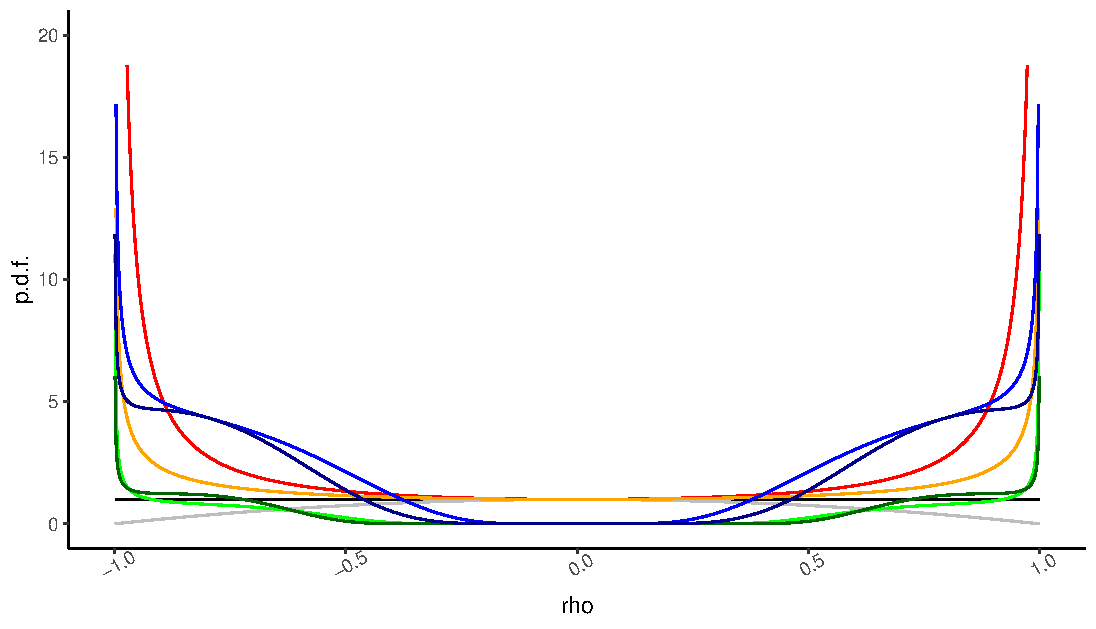
\includegraphics[width=0.85\linewidth]{prior_comparison.pdf}
	\caption{Different probability density functions for $\mu_j$ a)black for uniform distribution,
	b)grey for Beta(2,2),
	c)red for Jeffrey's prior,
	d)orange for Beta(0.5,0.5),
	e)green for inverse-gamma (1,1),
	f)dark green for inverse-gamma (2,2),
	g)blue for log-normal (0,1) and
	h)dark blue for log-normal (0, 0.8)}
	\label{fig:sim-prior}
\end{figure}
\fi

\section{Simulation Studies}

\subsection{Data generation}

To generate the true copula parameter, we first consider 4 different test cases to simulate Kendall's tau conditional on $x$. Such that
 
\begin{itemize}
    \item Case 1: True $\tau_x$ has a tree structure with respect to $x$. To obtain the tree structure we first generate a random binary tree such that number of terminal nodes is 8 and and difference between left and right terminal node is 4. Then we generate $\tau_x$ such that
    \begin{equation}
        \tau_x = \begin{cases}
        0.574 + \mathcal{N}(0,0.01) & x \le 0.251\\
        0.505 + \mathcal{N}(0,0.01) & 0.251 < x \le 0.267\\
        0.674 + \mathcal{N}(0,0.01) & 0.267 < x \le 0.308\\
        0.690 + \mathcal{N}(0,0.01) & 0.308 < x \le 0.312\\
        0.565 + \mathcal{N}(0,0.01) & 0.312 < x \le 0.361\\
        0.422 + \mathcal{N}(0,0.01) & 0.361 < x \le 0.538\\
        0.646 + \mathcal{N}(0,0.01) & 0.538 < x \le 0.933\\
        0.405 + \mathcal{N}(0,0.01) & 0.933 < x
    \end{cases}
    \end{equation}
    \item Case 2: True $\tau_x$ is monotone with respect to $x$ such that 
    \begin{equation}\label{eq:synth:tau_x:case2}
        \tau_x = 0.3 + 0.2 \sin(3x) + 0.3x^2.
    \end{equation}
    \item Case 3: True $\tau_x$ is convex with respect to $x$ such that 
    \begin{equation}\label{eq:synth:tau_x:case3}
        \tau_x = 0.5 + 0.3 \sin(3x).
    \end{equation}
    \item Case 4: True $\tau_x$ non-convex and non-monotone with respect to $x$ such that 
    \begin{equation}\label{eq:synth:tau_x:case4}
        \tau_x = 0.6 - 0.3 \sin(2x) + 0.2 \sin(4x) + 0.3 x^2.
    \end{equation}
\end{itemize}

We present the plot of true values of Kendall's $\tau$ with respect to $x$ in \cref{fig:true:tau}. Additionally, we provide the tree structure based $\tau_x$ in for clearer interpretation of the splitting rule.

\begin{figure}
    \centering
    \caption{Splitting rule for the tree based $\tau_x$}
    \label{fig:tau_tree_split}
    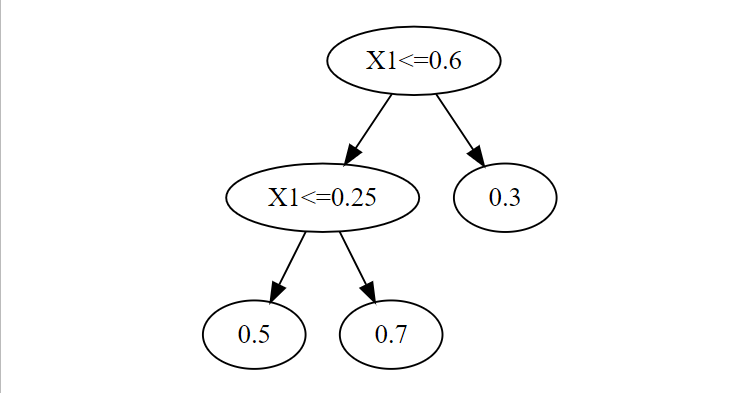
\includegraphics[width=0.5\linewidth]{tree_cond_tau_x.png}
\end{figure}

\begin{figure}
    \centering
    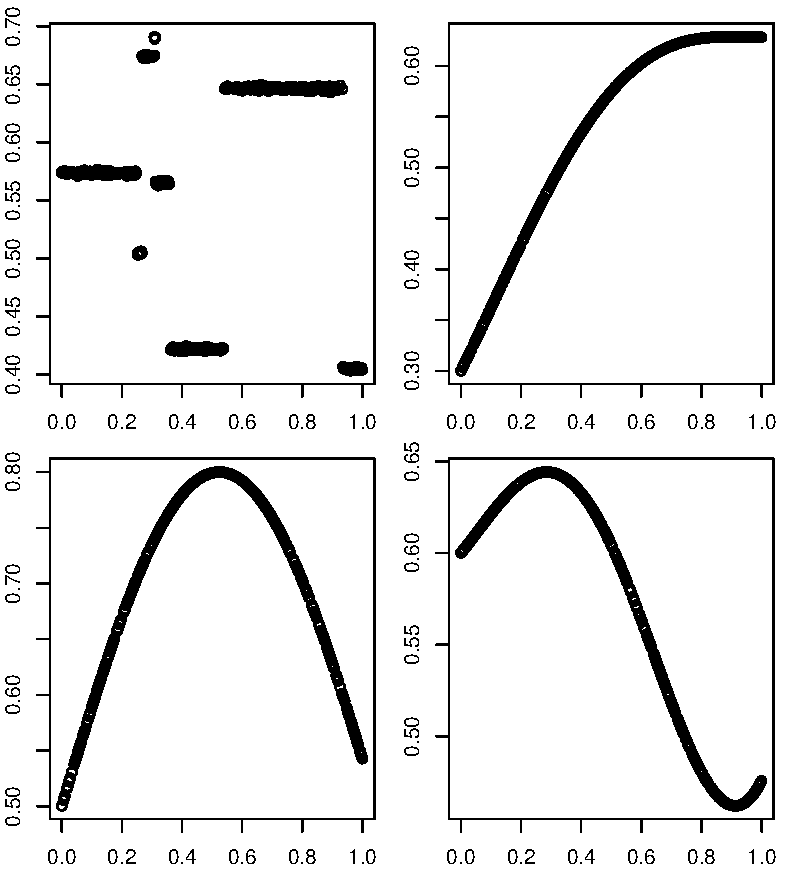
\includegraphics[width=0.95\linewidth]{true_tau.pdf}
    \caption{True values of Kendall's $\tau$ with respect to $x$. The top left plot shows case with tree structure; top right plot shows case defined by \cref{eq:synth:tau_x:case2}; bottom left shows case defined by \cref{eq:synth:tau_x:case3}; and bottom right shows case defined by \cref{eq:synth:tau_x:case4}.}
    \label{fig:true:tau}
\end{figure}

Then using these values of conditional Kendall's $\tau$, we generate the copula parameters using the link functions summarised in \cref{tab:cop:link}. Afterwards, we simulate from the copula density functions to obtain our synthetic dataset.

\begin{table}
    \centering
    \begin{tabular}{l|c|c|c}
    \toprule
        Family & Support & Relation with $\tau$ & Range of $\tau$ \\
         \midrule
        Gaussian & $\rho \in (-1,1)$ & $\sin(\tau\pi/2)$ & (-1,1)\\
        Student-t & $\rho \in (-1,1)$ & $\sin(\tau\pi/2)$ & (-1,1) \\
        Clayton & $\theta \in (0,\infty)$ & $2\tau/(1-\tau)$ & $(0,1)$ \\
        Gumbel & $\theta\in [1,\infty)$ & $1/(1-\tau)$  & $[0,1)$ \\
        \bottomrule
    \end{tabular}
    \caption{Copula families used for analyses, along with parameter support and relation with Kendall's $\tau$.}
    \label{tab:cop:link}
\end{table}

\paragraph{Prediction accuracy} For the sake of evaluating the efficiency of copula parameter estimation we check in sample prediction of the copula parameter ($\rho$ for Gaussian and student-t; $\theta$ for Clayton and Gumbel) using the posterior samples of the regression trees . 

There after we check the root mean squared error with respect to the true copula parameter used in the data generation phase. Given by:

\begin{equation}
    \text{RMSE} = \sqrt{1/n\sum_{i=1}^n (\theta_i - \overline{\theta}^*_i)^2}
\end{equation}
where $\overline{\theta}^*_i$ is posterior sample mean of copula parameter conditional on $x_i$.

For credible interval coverage, check whether the true copula parameter is contained within the 95\% credible interval of the predictive samples of the copula parameter

\begin{equation}
    \text{CI coverage} = \frac{\sum_{i=1}^n\mathbb{I}\left(Q_{2.5}(\theta^*_i) \le \theta_i \le Q_{97.5}(\theta^*_i)\right)}{n}.
\end{equation}

Additionally, we check for credible interval length using $\left(Q_{97.5}(\theta^*_i) - Q_{2.5}(\theta^*_i)\right)$.

\subsection{Results}

\subsubsection{Gaussian Copula} For the Gaussian copula, the copula parameter $\rho$ lies within the open interval $(-1,1)$. So a natural choice for prior on $\mu_j$ is transformed beta as suggested by \citet{gokhale_prior_cor}. 

\begin{equation}
	\text{TBeta}(a, b) = \frac{1}{2^{a+b-1}\mathcal{B}(a,b)}(1+\rho)^{a-1}(1-\rho)^{b-1}\propto(1+\rho)^{a-1}(1-\rho)^{b-1},
\end{equation}
for $a,b>0$ and $\mathcal{B}$ denotes beta function. Note that, for $a=b=0$, this leads to an improper prior given by:
\begin{equation}
    \pi(\rho) \propto \frac{1}{(1-\rho)(1+\rho)}.
\end{equation}
This corresponds to the Jeffrey's prior as suggested by \citet{berger_2008_objective}.

From an implementation perspective, we only require $(1+\rho)^{a-1}(1-\rho)^{b-1}$ to evaluate the prior for MH algorithm. Therefore, setting $a=0, b=0$ in the transformed beta prior will allow us to analyse results for Jeffrey's prior. Sinilarly, setting $a=1,b=1$ will give us uniform prior on $\rho$.

We present the summary of our analyses with Gaussian copula in \cref{tab:gauss:summary}. 

\begin{table}[ht]
	\centering
	\caption{Summary of analyses with Gaussian copula. The columns represents the specific case, the type of prior on $\mu_j\mid T$, the posterior expected number of terminal nodes, the posterior expected depth, the acceptance rate of MH algorithm, RMSE of estimated $\rho$ against true $\rho$, length of credible interval and coverage frequency within the credible interval. The posterior quantities are obtained by running 15000 samples in a single chain, after that we remove 5000 samples and then it is thinned by 10.}
	\label{tab:gauss:summary}
	\scriptsize{
	\begin{tabular}{ll|cccccc}
		\toprule
		& Prior on $\mu_j$ & $\mathbb{E}(n_L\mid U,X)$ & $\mathbb{E}(D\mid U,X)$ & Acc. Rate & RMSE & CI length & CI coverage \\ 
		\midrule
		Case 1 & TBeta(0.5,0.5) & 4.538 & 2.403 & 0.2390 & 0.0096 & 0.1771 & 0.836 \\ 
		(Tree) & TBeta(0,0) & 4.862 & 2.607 & 0.2560 & 0.0089 & 0.1907 & 0.840 \\ 
		& TBeta(2,2) & 4.563 & 2.424 & 0.2420 & 0.0098 & 0.1948 & \textbf{0.908} \\ 
		& TBeta(1,1) & 4.608 & 2.484 & 0.2510 & 0.0092 & 0.1963 & 0.844 \\ 
		\midrule
		Case 2 & TBeta(0.5,0.5) & 3.176 & 1.814 & 0.2290 & 0.0021 & 0.1891 & 0.960 \\ 
		(\cref{eq:synth:tau_x:case2}) & TBeta(0,0) & 2.371 & 1.300 & 0.2130 & 0.0020 & 0.1592 & 0.968 \\ 
		& TBeta(2,2) & 2.522 & 1.390 & 0.2150 & 0.0020 & 0.1823 & \textbf{1.000} \\ 
		& TBeta(1,1) & 2.397 & 1.306 & 0.1900 & 0.0020 & 0.1625 & 0.930 \\ 
		\midrule
		Case 3 & TBeta(0.5,0.5) & 3.495 & 2.079 & 0.2410 & 0.0010 & 0.0743 & 0.760 \\ 
		(\cref{eq:synth:tau_x:case3}) & TBeta(0,0) & 3.863 & 2.165 & 0.2620 & 0.0009 & 0.0790 & \textbf{0.866} \\ 
		& TBeta(2,2) & 3.596 & 2.142 & 0.2460 & 0.0008 & 0.0808 & 0.790 \\ 
		& TBeta(1,1) & 5.374 & 2.966 & 0.3510 & 0.0009 & 0.0863 & 0.776 \\ 
		\midrule
		Case 4 & TBeta(0.5,0.5) & 2.558 & 1.402 & 0.2190 & 0.0005 & 0.1197 & \textbf{1.000} \\ 
		(\cref{eq:synth:tau_x:case4}) & TBeta(0,0) & 2.934 & 1.632 & 0.2520 & 0.0006 & 0.1227 & 0.972 \\ 
		& TBeta(2,2) & 2.398 & 1.308 & 0.2390 & 0.0005 & 0.1160 & 0.998 \\ 
		& TBeta(1,1) & 2.848 & 1.571 & 0.2120 & 0.0006 & 0.1296 & \textbf{1.000} \\ 
		\end{tabular}}
\end{table}

\paragraph{Convergence Diagnostic}
\begin{table}[ht]
	\centering
	\caption{Posterior convergence diagnostic for Gaussian copula. The first two columns represent the specific case, type of prior on $\mu_j\mid T$. Followed by auto-correlation (lag-1) denoted by `AC', effective sample size percentage denoted by `ESS (\%)' and Geweke score of posterior samples of depth, posterior samples of the number of terminal nodes and likelihood. To obtain the reduced samples we discard 5000 burnin samples followed by thinning of 10.}
	\scriptsize{
		\begin{tabular}{ll|crr|crr|crr}
			\toprule
			\multicolumn{2}{c|}{} &
			\multicolumn{3}{c|}{Depth} &
			\multicolumn{3}{c|}{$n_L$} &
			\multicolumn{3}{c}{likelihood} \\
			\midrule
			& Prior & AC & ESS (\%) & Geweke & AC & ESS (\%) & Geweke & AC & ESS (\%) & Geweke \\ 
			\midrule
			Case 1 & TBeta(1,1) & 0.95 & 0.82 & 5.23 & 0.96 & 1.46 & 1.42 & 0.88 & 1.85 & 3.09 \\ 
			all sample & TBeta(0.5,0.5) & 0.91 & 3.00 & -1.27 & 0.94 & 2.59 & -2.10 & 0.79 & 5.19 & -0.27 \\ 
			& TBeta(0,0) & 0.94 & 1.64 & -3.64 & 0.96 & 1.77 & -3.47 & 0.80 & 3.35 & 1.17 \\ 
			& TBeta(2,2) & 0.92 & 2.24 & -2.44 & 0.95 & 2.07 & -2.49 & 0.81 & 4.06 & 4.62 \\ 
			\midrule
			reduced sample & TBeta(1,1) & 0.63 & 5.34 & -1.80 & 0.66 & 8.63 & -1.56 & 0.56 & 19.99 & -0.06 \\ 
			& TBeta(0.5,0.5) & 0.56 & 13.42 & 0.06 & 0.61 & 12.42 & -0.01 & 0.13 & 26.78 & -1.47 \\ 
			& TBeta(0,0) & 0.66 & 12.67 & 0.22 & 0.70 & 11.99 & 0.12 & 0.19 & 13.06 & 0.81 \\ 
			& TBeta(2,2) & 0.58 & 8.92 & -1.52 & 0.65 & 10.25 & -2.30 & 0.29 & 29.62 & 1.10 \\ 
			\midrule
			Case 2 & TBeta(1,1) & 0.85 & 2.49 & -1.59 & 0.90 & 1.89 & -1.64 & 0.86 & 5.65 & 0.33 \\ 
			all sample & TBeta(0.5,0.5) & 0.96 & 0.13 & -1.57 & 0.98 & 0.14 & -1.72 & 0.94 & 0.58 & 1.03 \\ 
			& TBeta(0,0) & 0.83 & 4.58 & -1.93 & 0.89 & 3.48 & -2.01 & 0.69 & 14.52 & -1.31 \\ 
			& TBeta(2,2) & 0.87 & 2.24 & -3.88 & 0.92 & 1.70 & -3.75 & 0.69 & 14.77 & -0.06 \\ 
			\midrule
			reduced sample & TBeta(1,1) & 0.50 & 9.16 & -0.24 & 0.58 & 8.27 & 0.10 & 0.39 & 39.46 & -0.57 \\ 
			& TBeta(0.5,0.5) & 0.89 & 0.31 & -1.04 & 0.92 & 0.67 & -1.33 & 0.82 & 7.19 & 0.98 \\ 
			& TBeta(0,0) & 0.31 & 33.88 & -2.14 & 0.44 & 28.33 & -1.80 & 0.11 & 80.77 & -0.67 \\ 
			& TBeta(2,2) & 0.50 & 11.85 & -1.97 & 0.62 & 6.22 & -1.76 & 0.12 & 86.78 & 0.18 \\ 
			\midrule
			Case 3 & TBeta(1,1) & 0.97 & 0.33 & -1.83 & 0.98 & 0.52 & -2.16 & 0.98 & 0.51 & 2.67 \\ 
			all sample & TBeta(0.5,0.5) & 0.88 & 3.32 & 0.96 & 0.92 & 3.44 & 1.47 & 0.95 & 0.70 & 2.91 \\ 
			& TBeta(0,0) & 0.89 & 4.06 & -1.81 & 0.94 & 2.34 & -3.63 & 0.92 & 1.50 & 0.23 \\ 
			& TBeta(2,2) & 0.95 & 1.10 & 9.28 & 0.95 & 1.76 & 7.14 & 0.90 & 2.86 & -1.19 \\ 
			\midrule
			reduced sample & TBeta(1,1) & 0.83 & 1.09 & 2.69 & 0.80 & 1.39 & 1.99 & 0.85 & 3.42 & -1.27 \\ 
			& TBeta(0.5,0.5) & 0.26 & 59.01 & 0.21 & 0.40 & 38.65 & -0.32 & 0.41 & 41.89 & 0.32 \\ 
			& TBeta(0,0) & 0.35 & 36.00 & 0.09 & 0.57 & 17.03 & 0.69 & 0.67 & 5.15 & -1.88 \\ 
			& TBeta(2,2) & 0.47 & 30.46 & 1.26 & 0.51 & 28.39 & 0.88 & 0.40 & 16.41 & -0.83 \\  
			\midrule
			Case 4 & TBeta(1,1) & 0.97 & 0.34 & 2.75 & 0.97 & 0.45 & 3.02 & 0.98 & 0.70 & -0.35 \\ 
			all sample & TBeta(0.5,0.5) & 0.90 & 3.06 & 0.40 & 0.93 & 2.45 & 0.45 & 0.95 & 0.62 & 1.36 \\ 
			& TBeta(0,0) & 0.90 & 5.05 & 0.64 & 0.93 & 3.21 & -0.18 & 0.87 & 2.03 & 1.02 \\ 
			& TBeta(2,2) & 0.91 & 4.00 & 0.24 & 0.94 & 3.01 & 0.89 & 0.78 & 4.65 & -1.33 \\ 
			\midrule
			reduced sample & TBeta(1,1) & 0.78 & 1.28 & 3.55 & 0.78 & 1.80 & 1.56 & 0.92 & 2.43 & 0.04 \\ 
			& TBeta(0.5,0.5) & 0.41 & 28.62 & 0.74 & 0.54 & 18.10 & 0.64 & 0.73 & 2.15 & -1.42 \\ 
			& TBeta(0,0) & 0.39 & 44.21 & 0.85 & 0.52 & 31.39 & 0.49 & 0.24 & 12.61 & 1.34 \\ 
			& TBeta(2,2) & 0.41 & 35.74 & -0.37 & 0.54 & 19.52 & -0.73 & 0.13 & 32.53 & 0.82 \\ 
			\midrule
	\end{tabular}}
\end{table}

\paragraph{Trace-plots} We present trace-plots for $n_l$, depth and likelihood for case 1 in \cref{fig:case1:gauss:nterm,fig:case1:gauss:depth,fig:case1:gauss:like}. Similarly for case 2 the trace-plots are provided in \cref{fig:case2:gauss:nterm,fig:case2:gauss:depth,fig:case2:gauss:like}; for case 3 the trace-plots are provided in \cref{fig:case3:gauss:nterm,fig:case3:gauss:depth,fig:case3:gauss:like}; and for case 4 the trace-plots are provided in \cref{fig:case4:gauss:nterm,fig:case4:gauss:depth,fig:case4:gauss:like}.

% Tbeta(2,2) seems to be good, acceptance rate is high and likelihood seems to be more consistent


\begin{figure}
	\centering
	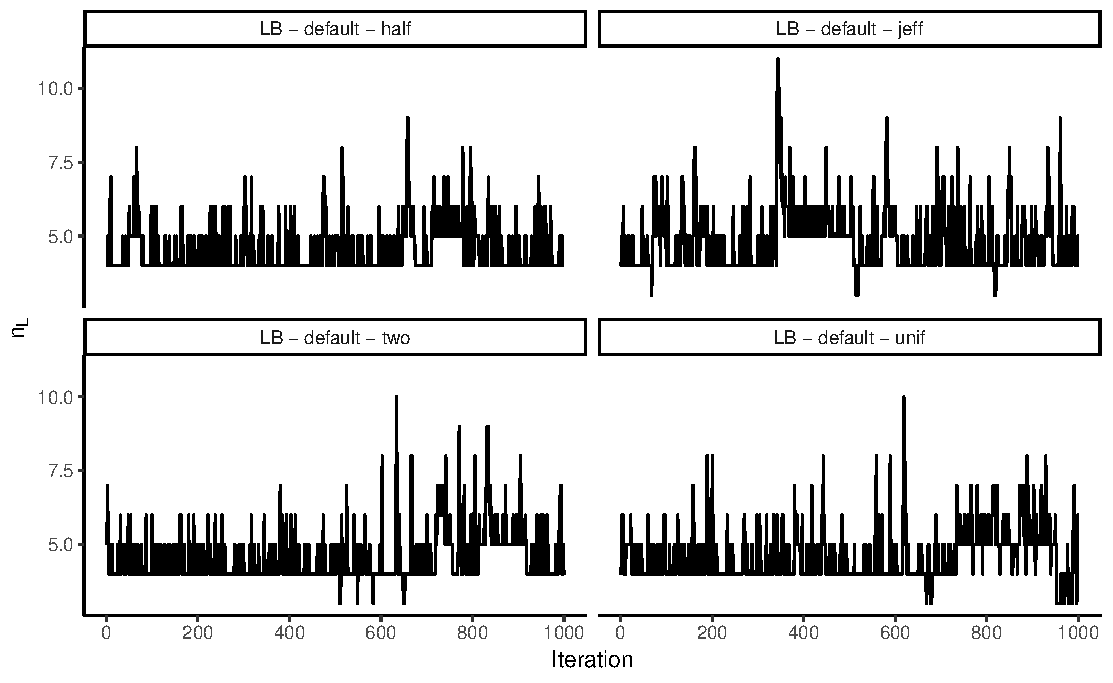
\includegraphics[width = 0.75\linewidth]{trace_case1_gauss_nterm.pdf}
	\caption{Trace plot of $n_L$ for case 1 (tree structure) with Gaussian copula. The top left denotes analysis with TBeta(0.5,0.5), top right denotes analysis with TBeta(0,0), bottom left denotes analysis with TBeta(2,2) and bottom right denotes analysis with TBeta(1,1).}
	\label{fig:case1:gauss:nterm}
\end{figure}

\begin{figure}
	\centering
	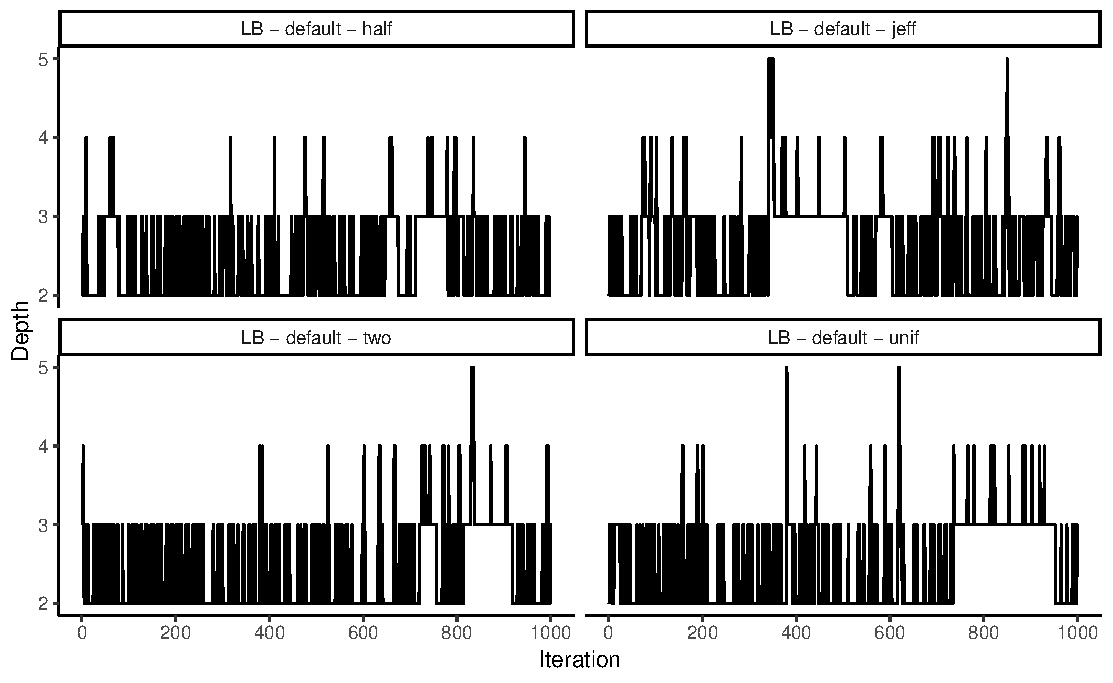
\includegraphics[width = 0.75\linewidth]{trace_case1_gauss_depth.pdf}
	\caption{Trace plot of depth for case 1 (tree structure) with Gaussian copula. The top left denotes analysis with TBeta(0.5,0.5), top right denotes analysis with TBeta(0,0), bottom left denotes analysis with TBeta(2,2) and bottom right denotes analysis with TBeta(1,1).}
	\label{fig:case1:gauss:depth}
\end{figure}

\begin{figure}
	\centering
	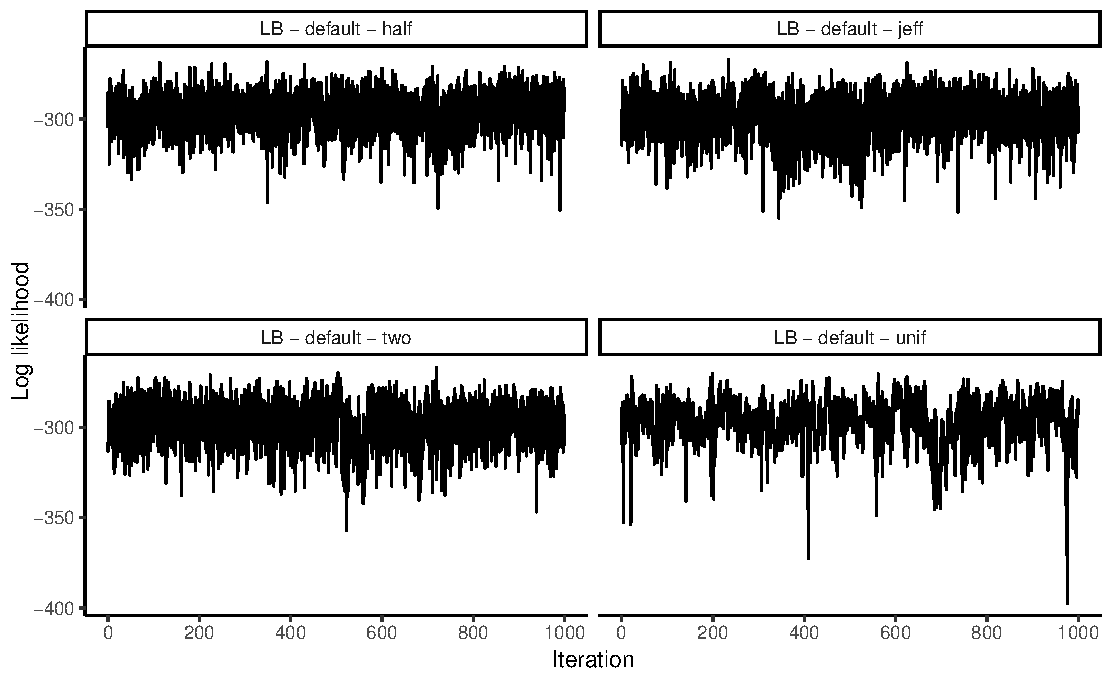
\includegraphics[width = 0.75\linewidth]{trace_case1_gauss_like.pdf}
	\caption{Trace plot of likelihood for case 1 (tree structure) with Gaussian copula. The top left denotes analysis with TBeta(0.5,0.5), top right denotes analysis with TBeta(0,0), bottom left denotes analysis with TBeta(2,2) and bottom right denotes analysis with TBeta(1,1).}
	\label{fig:case1:gauss:like}
\end{figure}

\begin{figure}
	\centering
	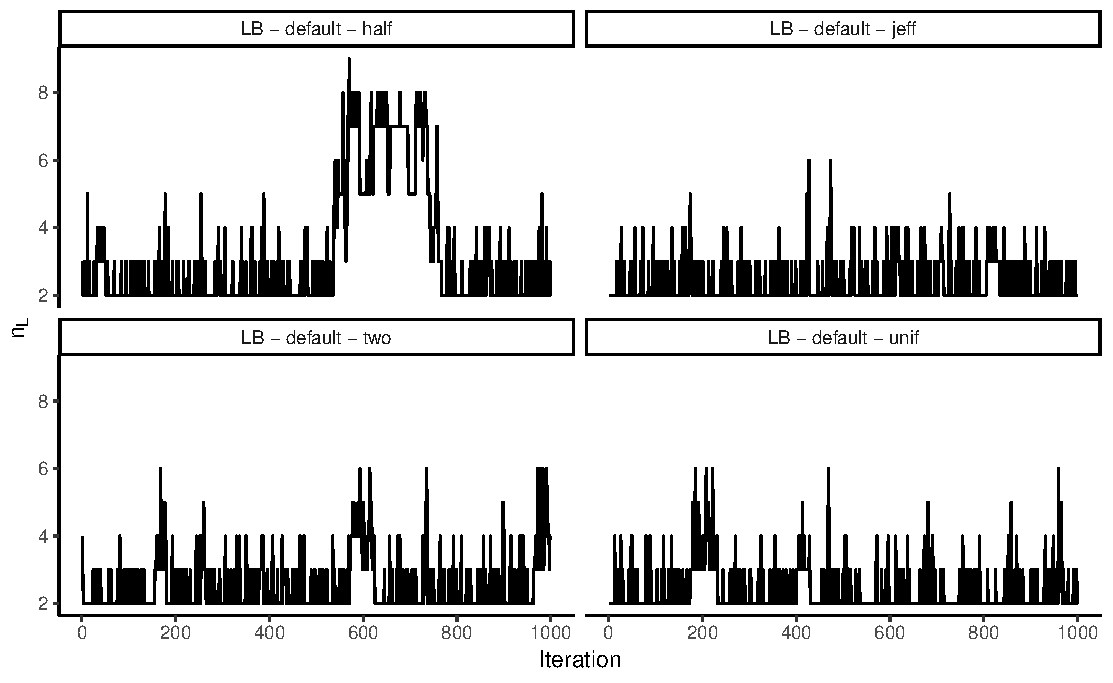
\includegraphics[width = 0.75\linewidth]{trace_case2_gauss_nterm.pdf}
	\caption{Trace plot of $n_L$ for case 2 (\cref{eq:synth:tau_x:case2}) with Gaussian copula. The top left denotes analysis with TBeta(0.5,0.5), top right denotes analysis with TBeta(0,0), bottom left denotes analysis with TBeta(2,2) and bottom right denotes analysis with TBeta(1,1).}
	\label{fig:case2:gauss:nterm}
\end{figure}

\begin{figure}
	\centering
	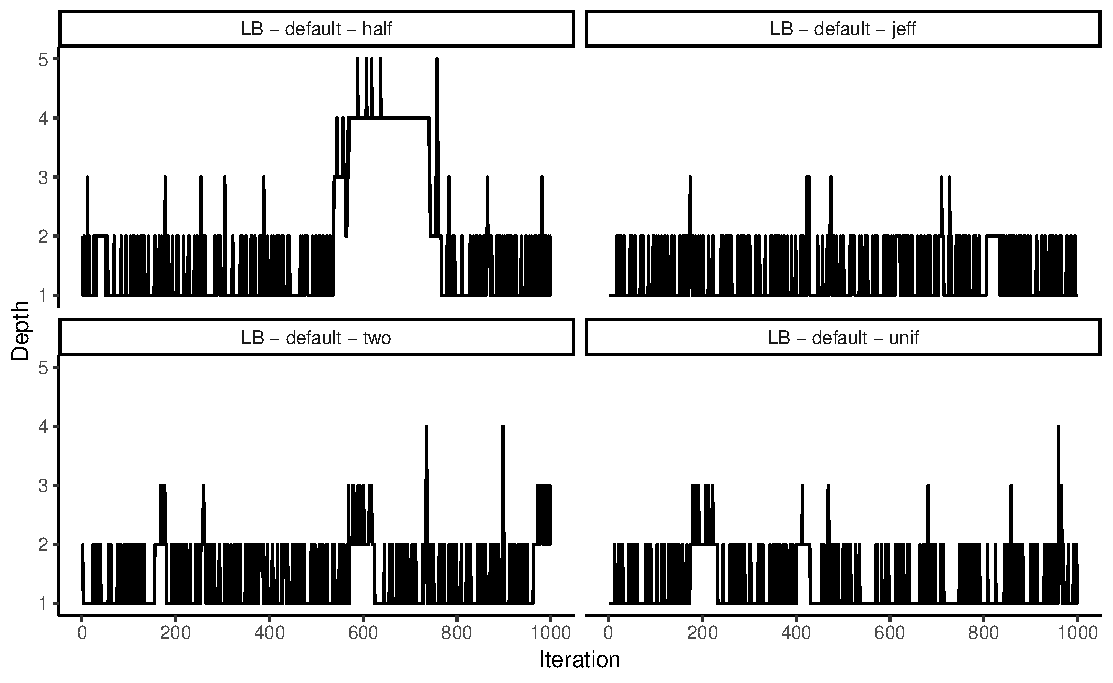
\includegraphics[width = 0.75\linewidth]{trace_case2_gauss_depth.pdf}
	\caption{Trace plot of depth for case 2 (\cref{eq:synth:tau_x:case2}) with Gaussian copula. The top left denotes analysis with TBeta(0.5,0.5), top right denotes analysis with TBeta(0,0), bottom left denotes analysis with TBeta(2,2) and bottom right denotes analysis with TBeta(1,1).}
	\label{fig:case2:gauss:depth}
\end{figure}

\begin{figure}
	\centering
	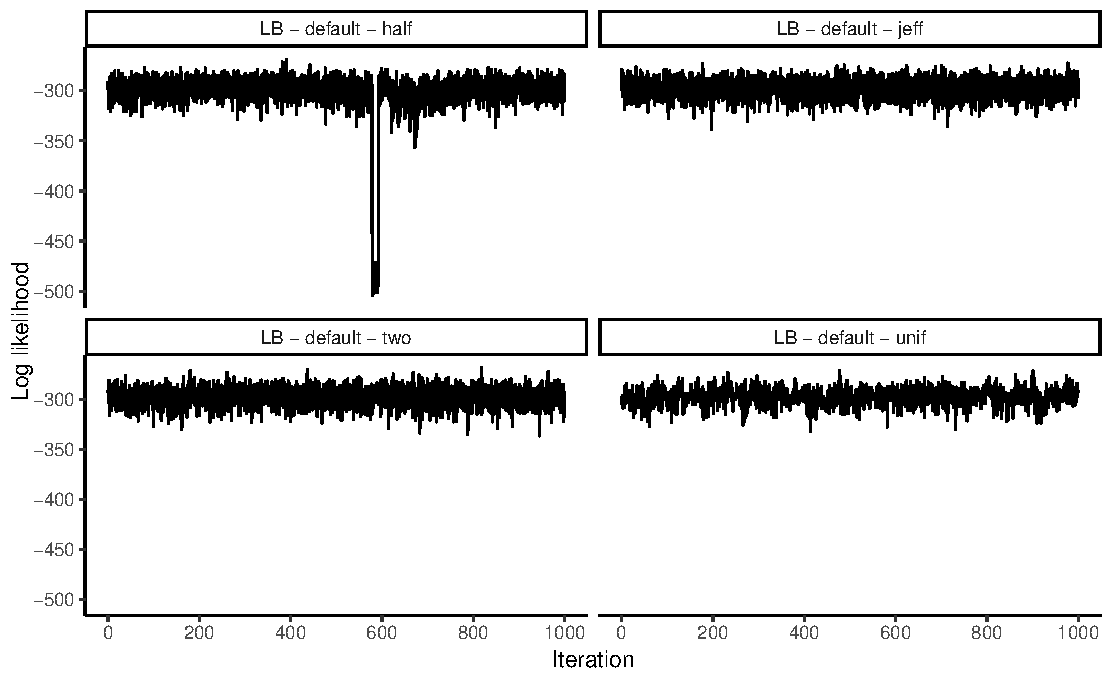
\includegraphics[width = 0.75\linewidth]{trace_case2_gauss_like.pdf}
	\caption{Trace plot of likelihood for case 2 (\cref{eq:synth:tau_x:case2}) with Gaussian copula. The top left denotes analysis with TBeta(0.5,0.5), top right denotes analysis with TBeta(0,0), bottom left denotes analysis with TBeta(2,2) and bottom right denotes analysis with TBeta(1,1).}
	\label{fig:case2:gauss:like}
\end{figure}

\begin{figure}
	\centering
	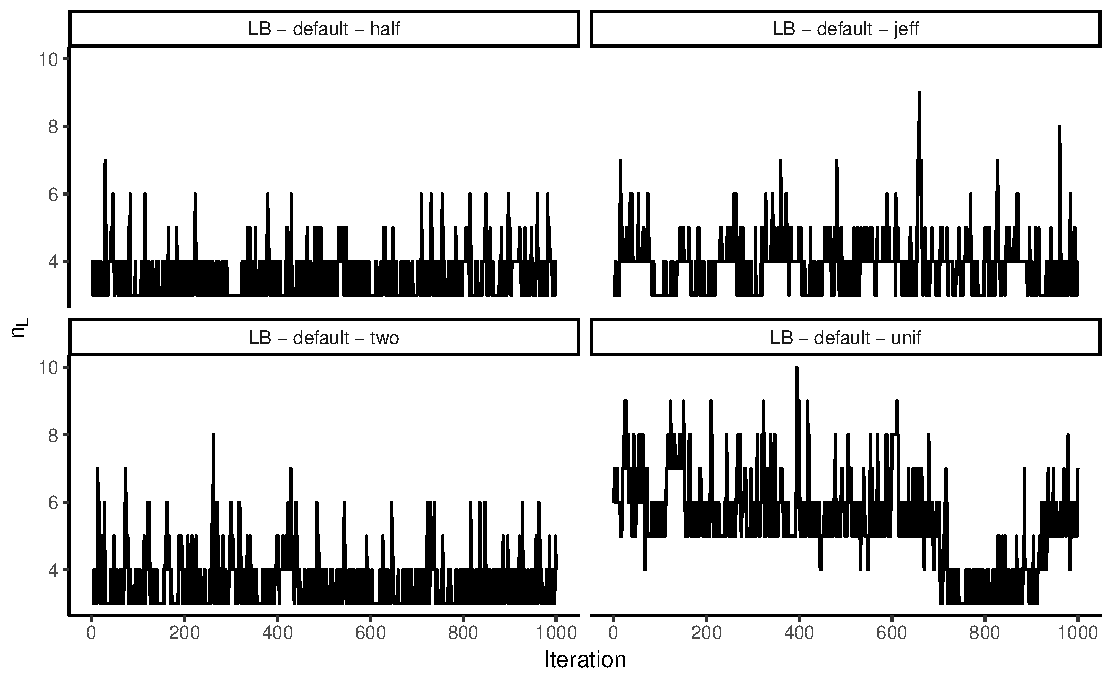
\includegraphics[width = 0.75\linewidth]{trace_case3_gauss_nterm.pdf}
	\caption{Trace plot of $n_L$ for case 3 (\cref{eq:synth:tau_x:case3}) with Gaussian copula. The top left denotes analysis with TBeta(0.5,0.5), top right denotes analysis with TBeta(0,0), bottom left denotes analysis with TBeta(2,2) and bottom right denotes analysis with TBeta(1,1).}
	\label{fig:case3:gauss:nterm}
\end{figure}

\begin{figure}
	\centering
	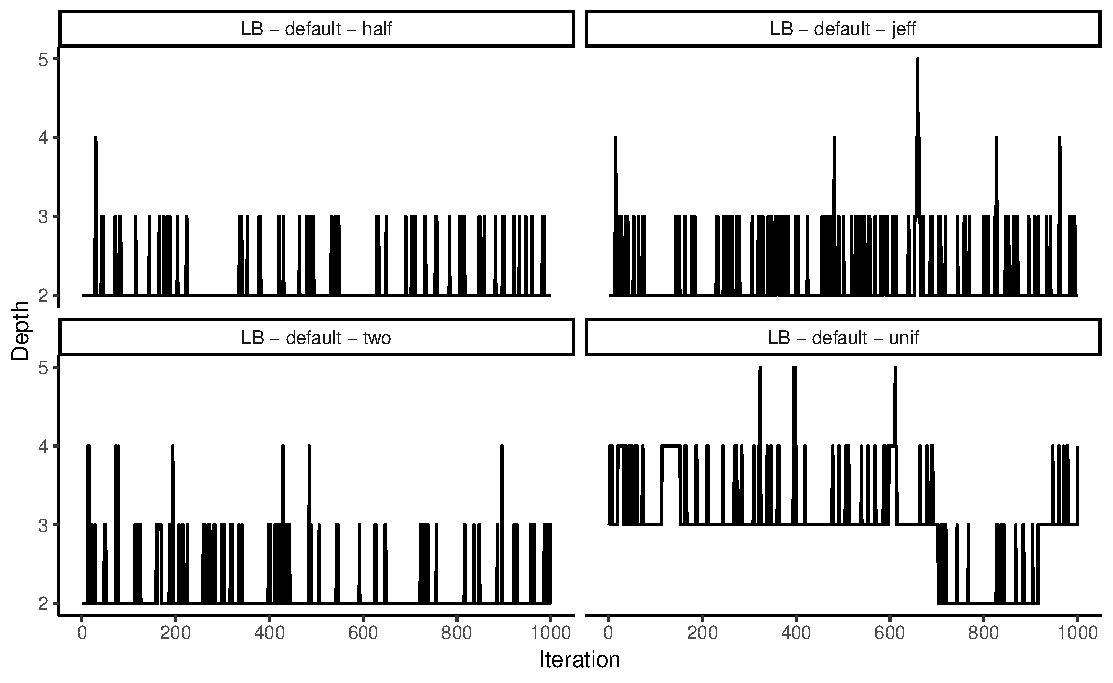
\includegraphics[width = 0.75\linewidth]{trace_case3_gauss_depth.pdf}
	\caption{Trace plot of depth for case 3 (\cref{eq:synth:tau_x:case3}) with Gaussian copula. The top left denotes analysis with TBeta(0.5,0.5), top right denotes analysis with TBeta(0,0), bottom left denotes analysis with TBeta(2,2) and bottom right denotes analysis with TBeta(1,1).}
	\label{fig:case3:gauss:depth}
\end{figure}

\begin{figure}
	\centering
	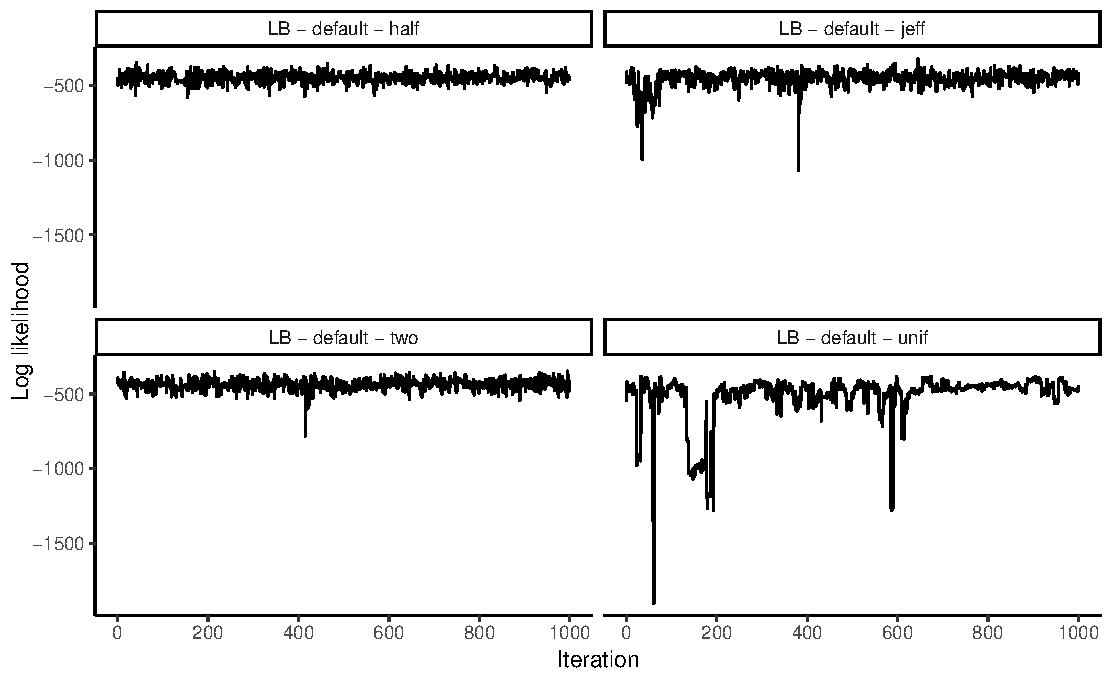
\includegraphics[width = 0.75\linewidth]{trace_case3_gauss_like.pdf}
	\caption{Trace plot of likelihood for case 3 (\cref{eq:synth:tau_x:case3}) with Gaussian copula. The top left denotes analysis with TBeta(0.5,0.5), top right denotes analysis with TBeta(0,0), bottom left denotes analysis with TBeta(2,2) and bottom right denotes analysis with TBeta(1,1).}
	\label{fig:case3:gauss:like}
\end{figure}

\begin{figure}
	\centering
	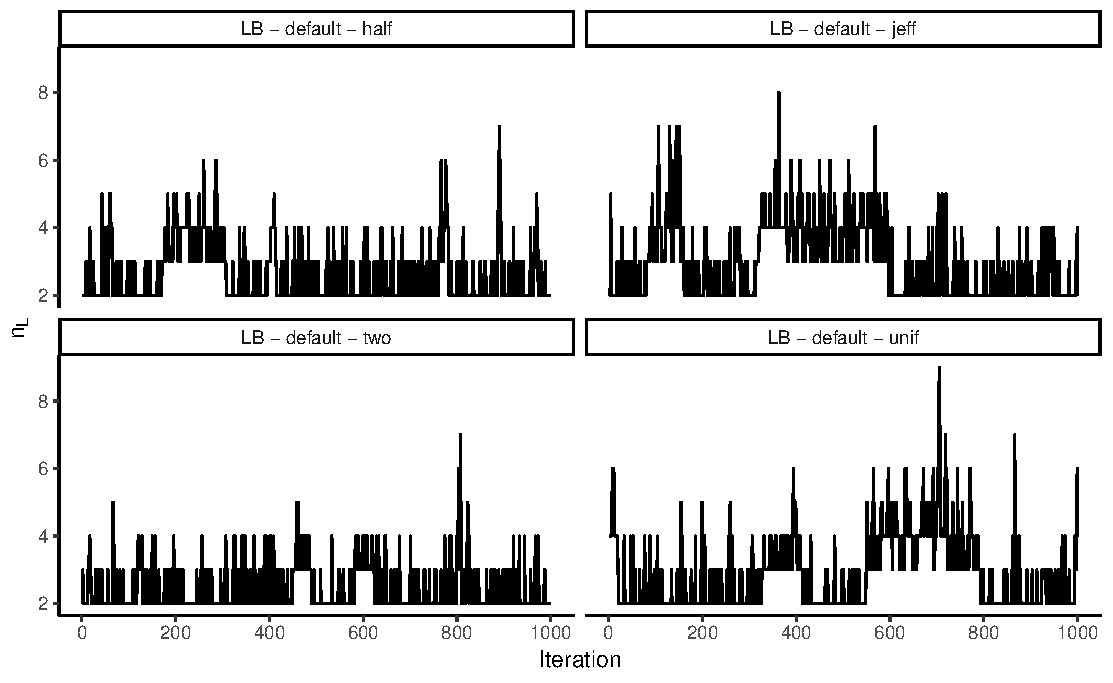
\includegraphics[width = 0.75\linewidth]{trace_case4_gauss_nterm.pdf}
	\caption{Trace plot of $n_L$ for case 4 (\cref{eq:synth:tau_x:case4}) with Gaussian copula. The top left denotes analysis with TBeta(0.5,0.5), top right denotes analysis with TBeta(0,0), bottom left denotes analysis with TBeta(2,2) and bottom right denotes analysis with TBeta(1,1).}
	\label{fig:case4:gauss:nterm}
\end{figure}

\begin{figure}
	\centering
	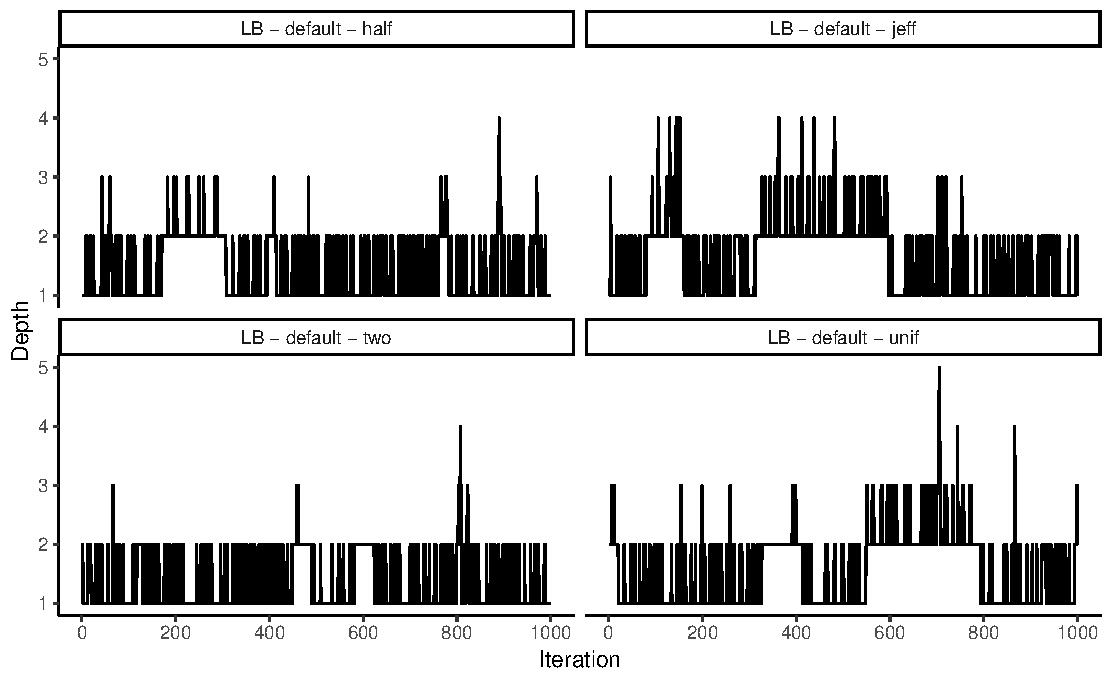
\includegraphics[width = 0.75\linewidth]{trace_case4_gauss_depth.pdf}
	\caption{Trace plot of depth for case 4 (\cref{eq:synth:tau_x:case4}) with Gaussian copula. The top left denotes analysis with TBeta(0.5,0.5), top right denotes analysis with TBeta(0,0), bottom left denotes analysis with TBeta(2,2) and bottom right denotes analysis with TBeta(1,1).}
	\label{fig:case4:gauss:depth}
\end{figure}

\begin{figure}
	\centering
	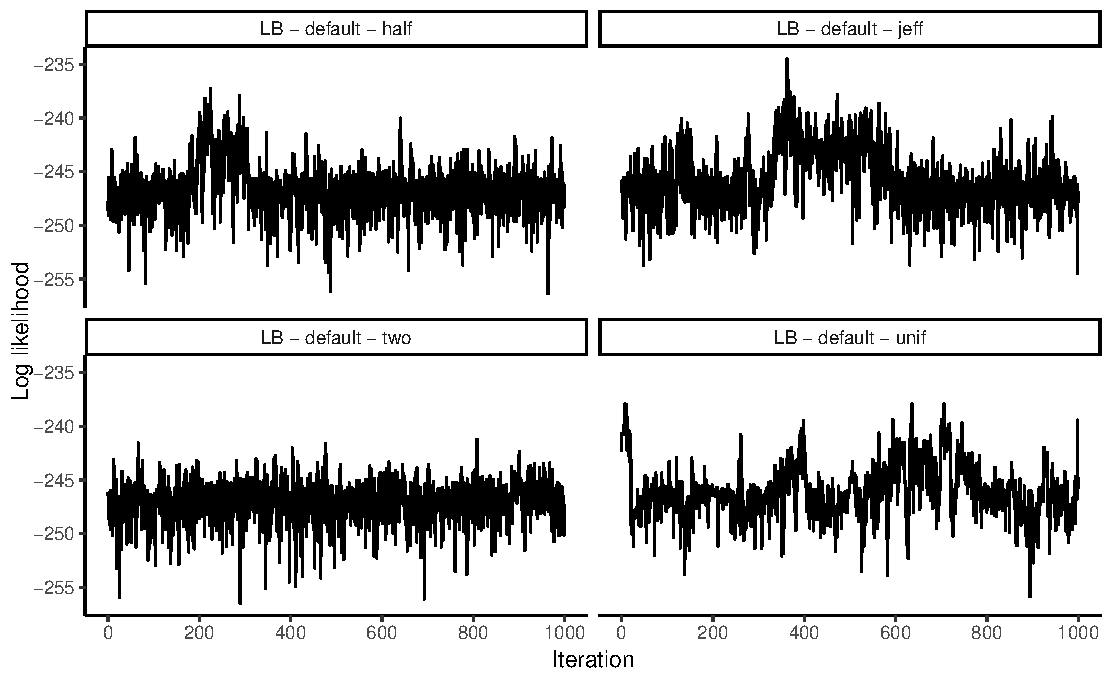
\includegraphics[width = 0.75\linewidth]{trace_case4_gauss_like.pdf}
	\caption{Trace plot of likelihood for case 4 (\cref{eq:synth:tau_x:case4}) with Gaussian copula. The top left denotes analysis with TBeta(0.5,0.5), top right denotes analysis with TBeta(0,0), bottom left denotes analysis with TBeta(2,2) and bottom right denotes analysis with TBeta(1,1).}
	\label{fig:case4:gauss:like}
\end{figure}

\subsubsection{Student-t copula} For the student-t copula we are only interested in estimating $\rho$ which lies within $(-1,1)$. Therefore, similar to Gaussian copula, we use a transformed beta distribution as a prior on $\mu_j$ with four different sets of parameters.

We present the summary of our analyses with student-t copula in \cref{tab:student-t:summary}. 


\begin{table}[ht]
	\centering
	\caption{Summary of analyses with student-t copula. The columns represents the specific case, the type of prior on $\mu_j\mid T$, the posterior expected number of terminal nodes, the posterior expected depth, the acceptance rate of MH algorithm, RMSE of estimated $\rho$ against true $\rho$, length of credible interval and coverage frequency within the credible interval. The posterior quantities are obtained by running 15000 samples in a single chain, after that we remove 5000 samples and then it is thinned by 10.}
	\label{tab:student-t:summary}
	\scriptsize{
	\begin{tabular}{ll|cccccc}
		\toprule
		& Prior on $\mu_j$ & $\mathbb{E}(n_L\mid U,X)$ & $\mathbb{E}(D\mid U,X)$ & Acc. Rate & RMSE & CI length & CI coverage \\ 
		\midrule
		Case 1 & TBeta(0.5,0.5) & 3.370 & 1.884 & 0.251 & 0.0079 & 0.2277 & 0.860 \\ 
		(Tree) & TBeta(0,0) & 4.089 & 2.228 & 0.268 & 0.0072 & 0.2445 & 0.850 \\ 
		& TBeta(2,2) & 3.620 & 2.041 & 0.260 & 0.0080 & 0.2420 & \textbf{0.862} \\ 
		& TBeta(1,1) & 3.604 & 1.996 & 0.232 & 0.0080 & 0.2308 & 0.854 \\ 
		\midrule
		Case 2 & TBeta(0.5,0.5) & 2.394 & 1.311 & 0.246 & 0.0019 & 0.1980 & \textbf{1.000} \\ 
		(\cref{eq:synth:tau_x:case2}) & TBeta(0,0) & 2.326 & 1.255 & 0.203 & 0.0018 & 0.2000 & \textbf{1.000} \\ 
		& TBeta(2,2) & 2.470 & 1.351 & 0.236 & 0.0019 & 0.2115 & \textbf{1.000} \\ 
		& TBeta(1,1) & 2.354 & 1.289 & 0.213 & 0.0018 & 0.1950 & \textbf{1.000} \\ 
		\midrule
		Case 3 & TBeta(0.5,0.5) & 3.499 & 2.102 & 0.261 & 0.0008 & 0.0997 & 0.916 \\ 
		(\cref{eq:synth:tau_x:case3}) & TBeta(0,0) & 3.727 & 2.170 & 0.261 & 0.0007 & 0.0992 & 0.928 \\ 
		& TBeta(2,2) & 3.545 & 2.127 & 0.238 & 0.0007 & 0.1127 & 0.896 \\ 
		& TBeta(1,1) & 3.847 & 2.234 & 0.243 & 0.0008 & 0.0971 & \textbf{0.950} \\ 
		\midrule
		Case 4 & TBeta(0.5,0.5) & 2.560 & 1.431 & 0.241 & 0.0003 & 0.1552 & \textbf{1.000} \\ 
		(\cref{eq:synth:tau_x:case4}) & TBeta(0,0) & 2.387 & 1.311 & 0.275 & 0.0003 & 0.1406 & \textbf{1.000} \\ 
		& TBeta(2,2) & 2.689 & 1.488 & 0.266 & 0.0003 & 0.1648 & \textbf{1.000} \\ 
		& TBeta(1,1) & 2.824 & 1.568 & 0.259 & 0.0003 & 0.1482 & \textbf{1.000} \\ 
		\end{tabular}}
\end{table}

\paragraph{Convergence Diagnostic}
\begin{table}[ht]
	\centering
	\caption{Posterior convergence diagnostic for student t copula. The first two columns represent the specific case, type of prior on $\mu_j\mid T$. Followed by auto-correlation (lag-1) denoted by `AC', effective sample size percentage denoted by `ESS (\%)' and Geweke score of posterior samples of depth, posterior samples of the number of terminal nodes and likelihood. To obtain the reduced samples we discard 5000 burnin samples followed by thinning of 10.}
	\scriptsize{
	\begin{tabular}{ll|crr|crr|crr}
		\toprule
		\multicolumn{2}{c|}{} &
		\multicolumn{3}{c|}{Depth} &
		\multicolumn{3}{c|}{$n_L$} &
		\multicolumn{3}{c}{likelihood} \\
		\midrule
		& Prior & AC & ESS (\%) & Geweke & AC & ESS (\%) & Geweke & AC & ESS (\%) & Geweke \\ 
		\midrule
		Case1 & TBeta(1,1) & 0.90 & 4 & -0.89 & 0.93 & 3 & -0.53 & 0.82 & 5 & 0.23 \\ 
		all sample & TBeta(0.5,0.5) & 0.91 & 3 & -3.10 & 0.95 & 2 & -2.92 & 0.84 & 4 & 1.57 \\ 
		& TBeta(0,0) & 0.92 & 3 & -3.67 & 0.95 & 2 & -3.56 & 0.87 & 2 & 1.48 \\ 
		& TBeta(2,2) & 0.92 & 2 & -4.31 & 0.95 & 1 & -3.67 & 0.83 & 5 & -0.18 \\ 
		\midrule
		reduced sample & TBeta(1,1) & 0.46 & 37 & 0.77 & 0.58 & 27 & 0.74 & 0.36 & 41 & 0.60 \\ 
		& TBeta(0.5,0.5) & 0.49 & 30 & 0.38 & 0.63 & 22 & 0.58 & 0.38 & 44 & -0.63 \\ 
		& TBeta(0,0) & 0.56 & 22 & 0.46 & 0.69 & 18 & 0.61 & 0.49 & 25 & 1.10 \\ 
		& TBeta(2,2) & 0.48 & 27 & -1.83 & 0.62 & 16 & -1.82 & 0.36 & 28 & 0.29 \\ 
		\midrule
		Case 2 & TBeta(1,1) & 0.94 & 1 & -2.64 & 0.97 & 1 & -2.87 & 0.86 & 5 & 2.83 \\ 
		all sample & TBeta(0.5,0.5) & 0.93 & 2 & 1.42 & 0.96 & 1 & 1.03 & 0.86 & 4 & 0.87 \\ 
		& TBeta(0,0) & 0.94 & 1 & -1.70 & 0.96 & 1 & -1.41 & 0.87 & 4 & 1.40 \\ 
		& TBeta(2,2) & 0.91 & 3 & 2.65 & 0.94 & 2 & 2.65 & 0.85 & 5 & 0.77 \\ 
		\midrule
		reduced sample & TBeta(1,1) & 0.66 & 6 & -0.27 & 0.77 & 4 & -0.60 & 0.43 & 34 & 1.08 \\ 
		& TBeta(0.5,0.5) & 0.60 & 14 & -1.19 & 0.74 & 12 & -1.36 & 0.34 & 37 & 0.05 \\ 
		& TBeta(0,0) & 0.68 & 7 & 0.94 & 0.76 & 8 & 1.13 & 0.45 & 32 & -0.07 \\ 
		& TBeta(2,2) & 0.44 & 30 & 1.32 & 0.54 & 30 & 0.49 & 0.35 & 34 & 0.79 \\ 
		\midrule
		Case 3 & TBeta(1,1) & 0.96 & 1 & -1.51 & 0.97 & 1 & -1.27 & 0.94 & 2 & 0.75 \\ 
		all sample & TBeta(0.5,0.5) & 0.98 & 1 & -3.07 & 0.99 & 1 & -3.19 & 0.94 & 2 & 2.07 \\ 
		& TBeta(0,0) & 0.95 & 1 & -1.90 & 0.97 & 1 & -2.42 & 0.95 & 2 & 1.68 \\ 
		& TBeta(2,2) & 0.95 & 1 & -0.80 & 0.97 & 1 & -1.21 & 0.94 & 2 & 1.29 \\ 
		\midrule
		reduced sample & TBeta(1,1) & 0.75 & 9 & 1.36 & 0.83 & 8 & 0.78 & 0.60 & 18 & 1.26 \\ 
		& TBeta(0.5,0.5) & 0.88 & 1 & -0.89 & 0.94 & 1 & -0.47 & 0.69 & 14 & -0.30 \\ 
		& TBeta(0,0) & 0.74 & 5 & 1.73 & 0.83 & 5 & 2.11 & 0.65 & 16 & 1.86 \\ 
		& TBeta(2,2) & 0.72 & 11 & 1.65 & 0.79 & 10 & 1.72 & 0.67 & 18 & 1.59 \\ 
		\midrule
		Case 4 & TBeta(1,1) & 0.95 & 1 & -0.39 & 0.97 & 1 & -0.24 & 0.91 & 1 & -1.65 \\ 
		all sample & TBeta(0.5,0.5) & 0.98 & 1 & -3.07 & 0.99 & 1 & -3.22 & 0.95 & 1 & -2.35 \\ 
		& TBeta(0,0) & 0.93 & 2 & -1.80 & 0.96 & 2 & -1.33 & 0.81 & 2 & -0.98 \\ 
		& TBeta(2,2) & 0.95 & 1 & -3.66 & 0.97 & 1 & -3.48 & 0.82 & 2 & -4.12 \\ 
		\midrule
		reduced sample & TBeta(1,1) & 0.74 & 6 & -2.17 & 0.83 & 5 & -2.28 & 0.87 & 4 & -2.48 \\ 
		& TBeta(0.5,0.5) & 0.88 & 1 & -1.47 & 0.94 & 1 & -2.03 & 0.94 & 1 & -1.33 \\ 
		& TBeta(0,0) & 0.57 & 20 & -0.52 & 0.69 & 15 & -0.53 & 0.64 & 15 & -2.28 \\ 
		& TBeta(2,2) & 0.72 & 9 & -0.16 & 0.83 & 9 & -0.29 & 0.70 & 14 & -0.04 \\ 
		\bottomrule
		\end{tabular}}
\end{table}

\paragraph{Trace-plots} We present trace-plots for $n_l$, depth and likelihood for case 1 in \cref{fig:case1:t:nterm,fig:case1:t:depth,fig:case1:t:like}. Similarly for case 2 the trace-plots are provided in \cref{fig:case2:t:nterm,fig:case2:t:depth,fig:case2:t:like}; for case 3 the trace-plots are provided in \cref{fig:case3:t:nterm,fig:case3:t:depth,fig:case3:t:like}; and for case 4 the trace-plots are provided in \cref{fig:case4:t:nterm,fig:case4:t:depth,fig:case4:t:like}.

% Tbeta(0,0) seems to be good, acceptance rate is high and likelihood seems to be more consistent

\begin{figure}
	\centering
	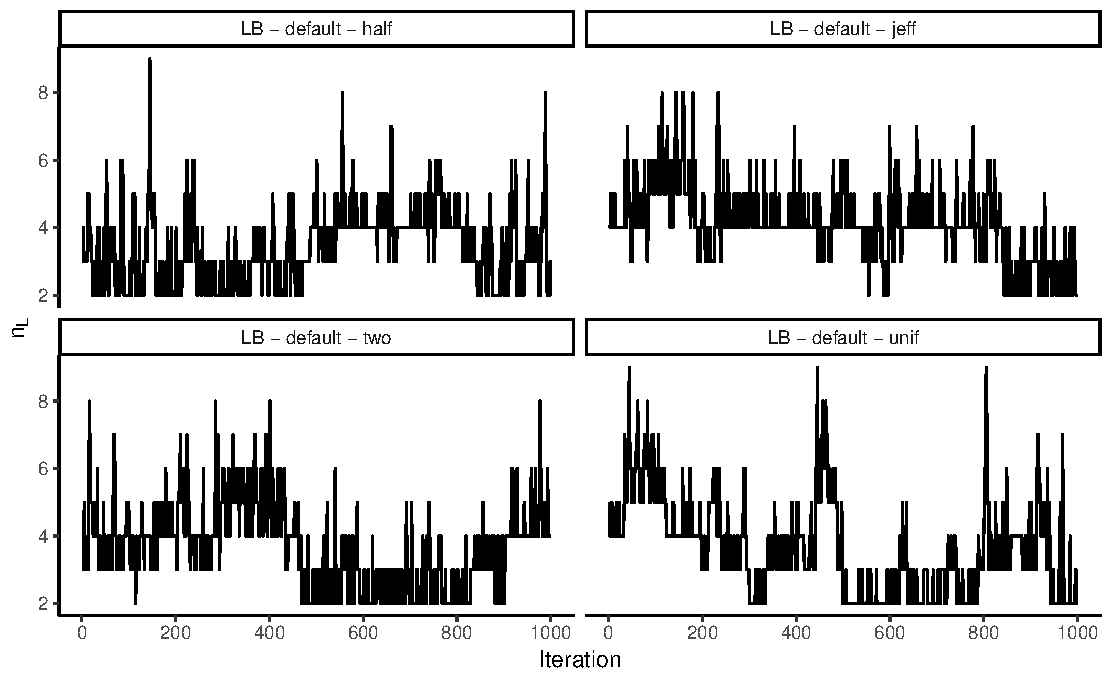
\includegraphics[width = 0.75\linewidth]{trace_case1_t_nterm.pdf}
	\caption{Trace plot of $n_L$ for case 1 (tree structure) with t copula. The top left denotes analysis with TBeta(0.5,0.5), top right denotes analysis with TBeta(0,0), bottom left denotes analysis with TBeta(2,2) and bottom right denotes analysis with TBeta(1,1).}
	\label{fig:case1:t:nterm}
\end{figure}

\begin{figure}
	\centering
	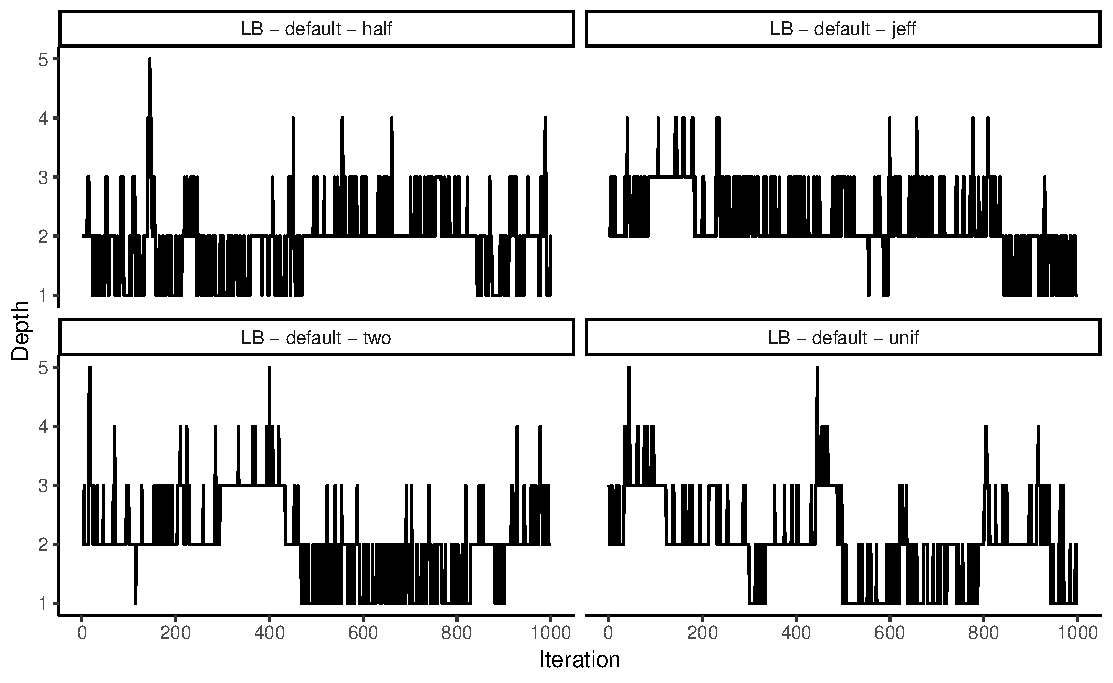
\includegraphics[width = 0.75\linewidth]{trace_case1_t_depth.pdf}
	\caption{Trace plot of depth for case 1 (tree structure) with t copula. The top left denotes analysis with TBeta(0.5,0.5), top right denotes analysis with TBeta(0,0), bottom left denotes analysis with TBeta(2,2) and bottom right denotes analysis with TBeta(1,1).}
	\label{fig:case1:t:depth}
\end{figure}

\begin{figure}
	\centering
	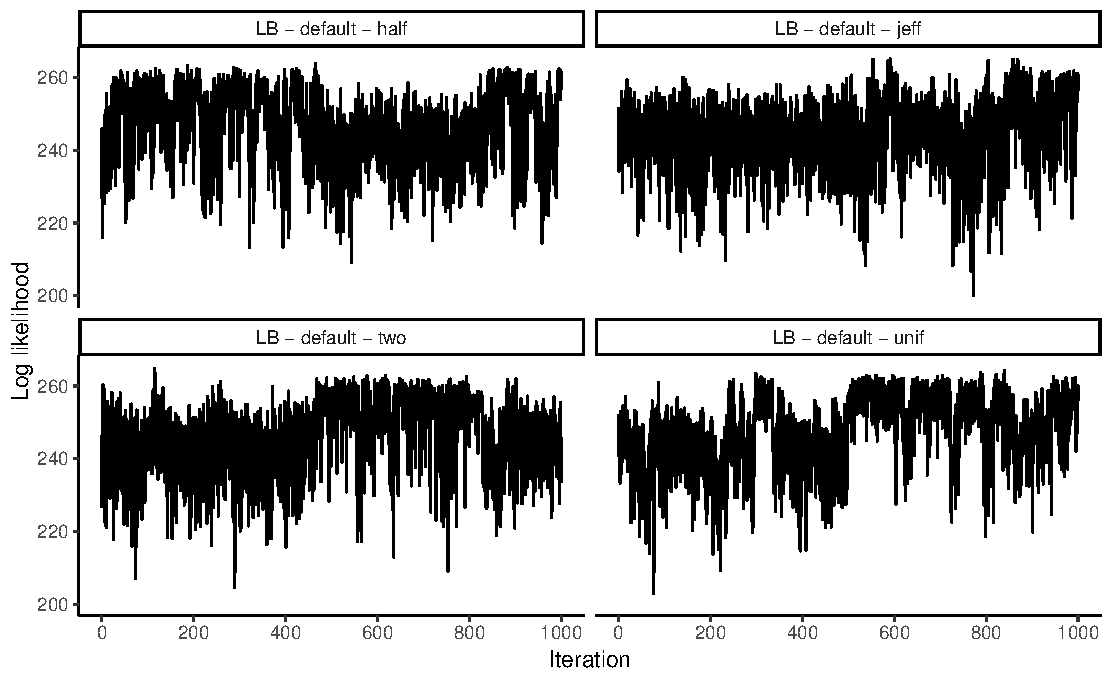
\includegraphics[width = 0.75\linewidth]{trace_case1_t_like.pdf}
	\caption{Trace plot of likelihood for case 1 (tree structure) with t copula. The top left denotes analysis with TBeta(0.5,0.5), top right denotes analysis with TBeta(0,0), bottom left denotes analysis with TBeta(2,2) and bottom right denotes analysis with TBeta(1,1).}
	\label{fig:case1:t:like}
\end{figure}

\begin{figure}
	\centering
	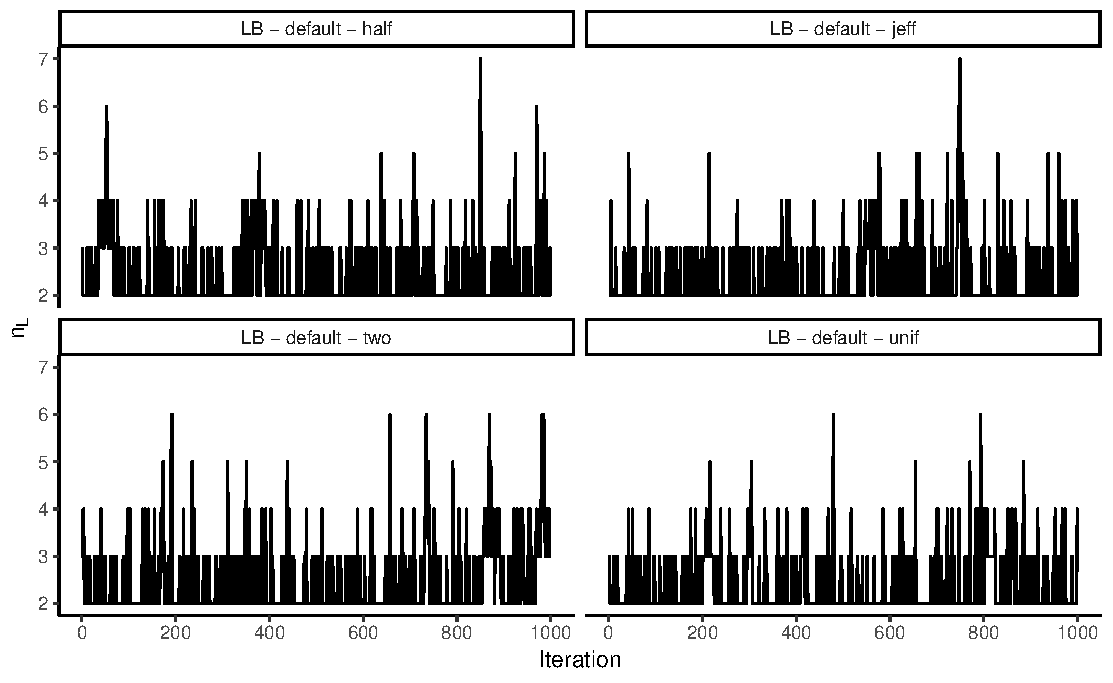
\includegraphics[width = 0.75\linewidth]{trace_case2_t_nterm.pdf}
	\caption{Trace plot of $n_L$ for case 2 (\cref{eq:synth:tau_x:case2}) with t copula. The top left denotes analysis with TBeta(0.5,0.5), top right denotes analysis with TBeta(0,0), bottom left denotes analysis with TBeta(2,2) and bottom right denotes analysis with TBeta(1,1).}
	\label{fig:case2:t:nterm}
\end{figure}

\begin{figure}
	\centering
	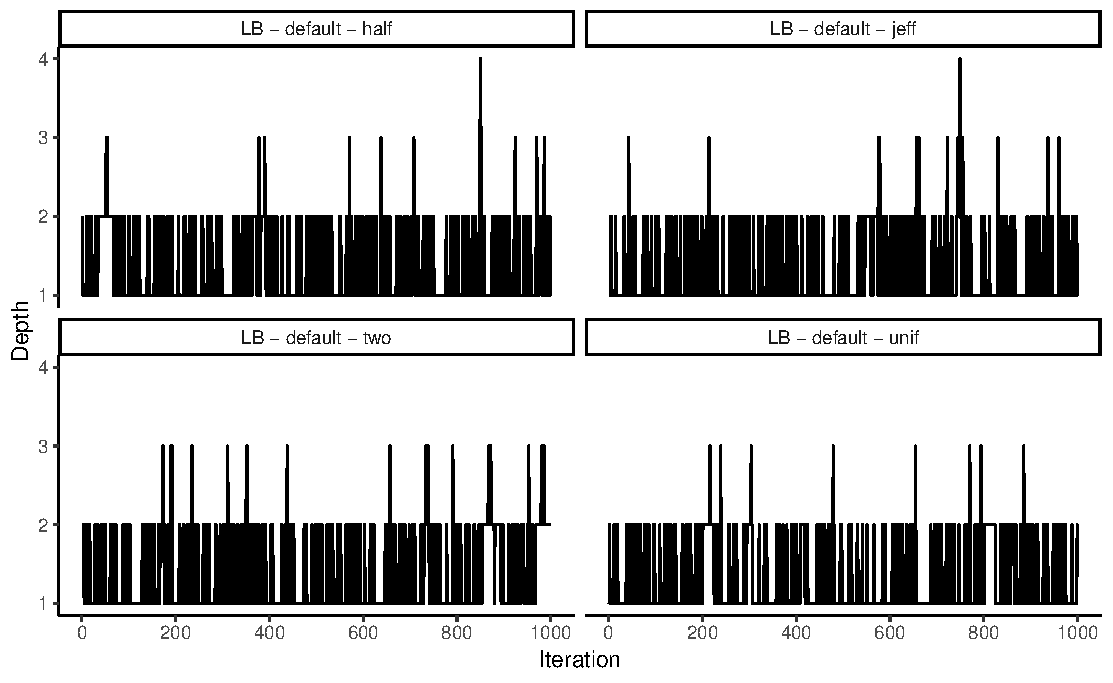
\includegraphics[width = 0.75\linewidth]{trace_case2_t_depth.pdf}
	\caption{Trace plot of depth for case 2 (\cref{eq:synth:tau_x:case2}) with t copula. The top left denotes analysis with TBeta(0.5,0.5), top right denotes analysis with TBeta(0,0), bottom left denotes analysis with TBeta(2,2) and bottom right denotes analysis with TBeta(1,1).}
	\label{fig:case2:t:depth}
\end{figure}

\begin{figure}
	\centering
	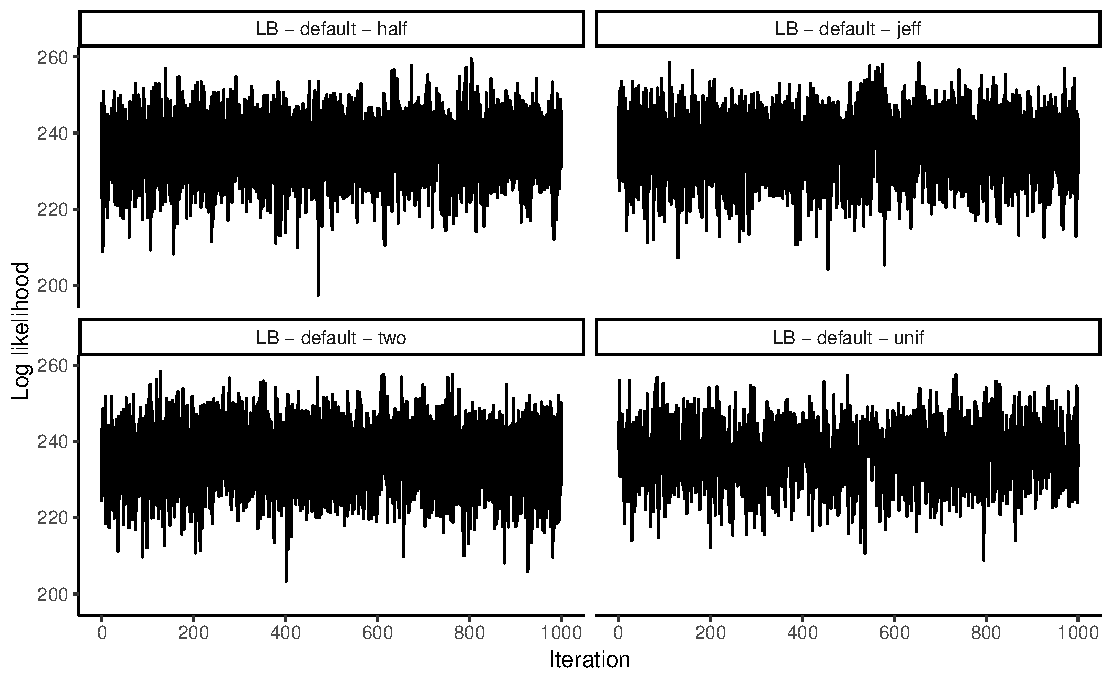
\includegraphics[width = 0.75\linewidth]{trace_case2_t_like.pdf}
	\caption{Trace plot of likelihood for case 2 (\cref{eq:synth:tau_x:case2}) with t copula. The top left denotes analysis with TBeta(0.5,0.5), top right denotes analysis with TBeta(0,0), bottom left denotes analysis with TBeta(2,2) and bottom right denotes analysis with TBeta(1,1).}
	\label{fig:case2:t:like}
\end{figure}

\begin{figure}
	\centering
	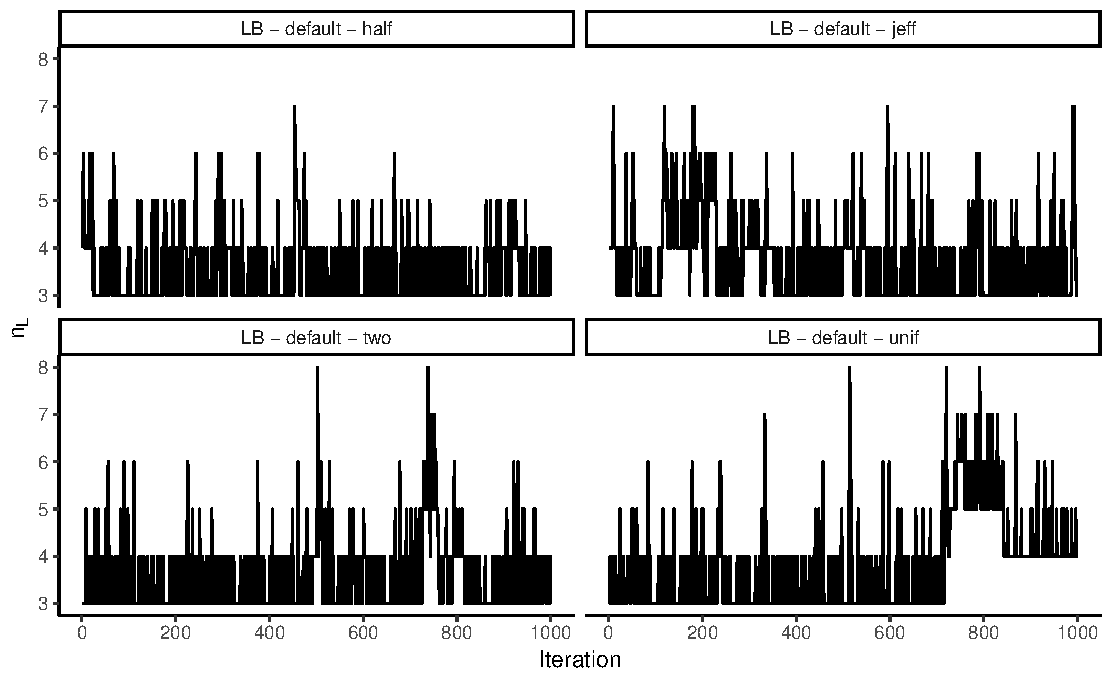
\includegraphics[width = 0.75\linewidth]{trace_case3_t_nterm.pdf}
	\caption{Trace plot of $n_L$ for case 3 (\cref{eq:synth:tau_x:case3}) with t copula. The top left denotes analysis with TBeta(0.5,0.5), top right denotes analysis with TBeta(0,0), bottom left denotes analysis with TBeta(2,2) and bottom right denotes analysis with TBeta(1,1).}
	\label{fig:case3:t:nterm}
\end{figure}

\begin{figure}
	\centering
	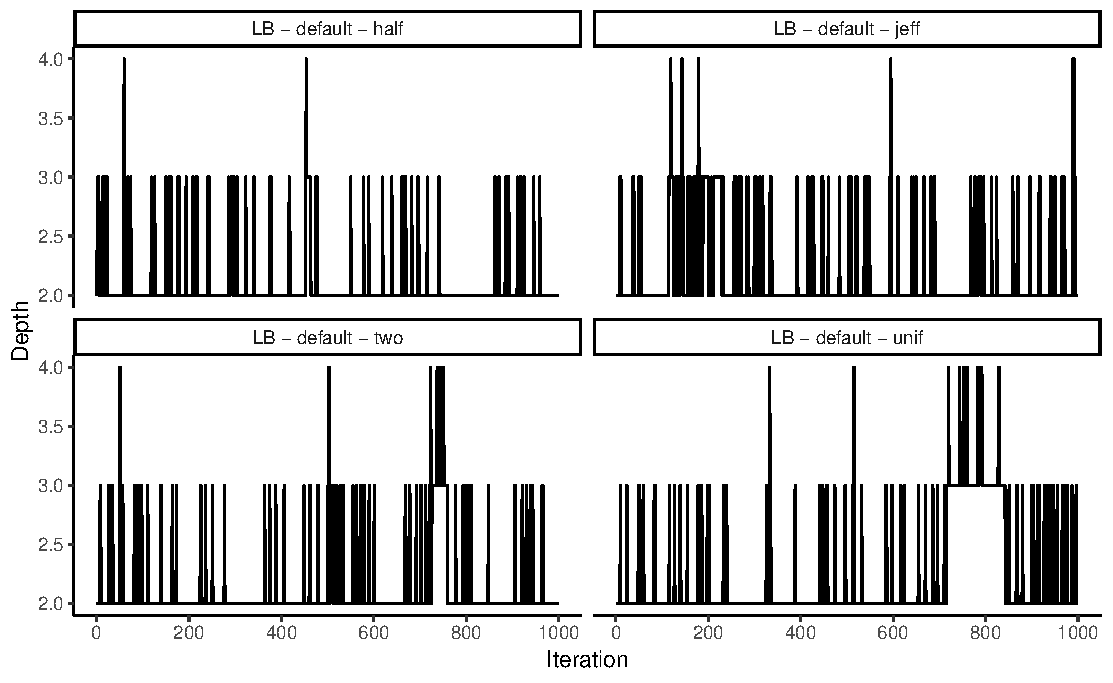
\includegraphics[width = 0.75\linewidth]{trace_case3_t_depth.pdf}
	\caption{Trace plot of depth for case 3 (\cref{eq:synth:tau_x:case3}) with t copula. The top left denotes analysis with TBeta(0.5,0.5), top right denotes analysis with TBeta(0,0), bottom left denotes analysis with TBeta(2,2) and bottom right denotes analysis with TBeta(1,1).}
	\label{fig:case3:t:depth}
\end{figure}

\begin{figure}
	\centering
	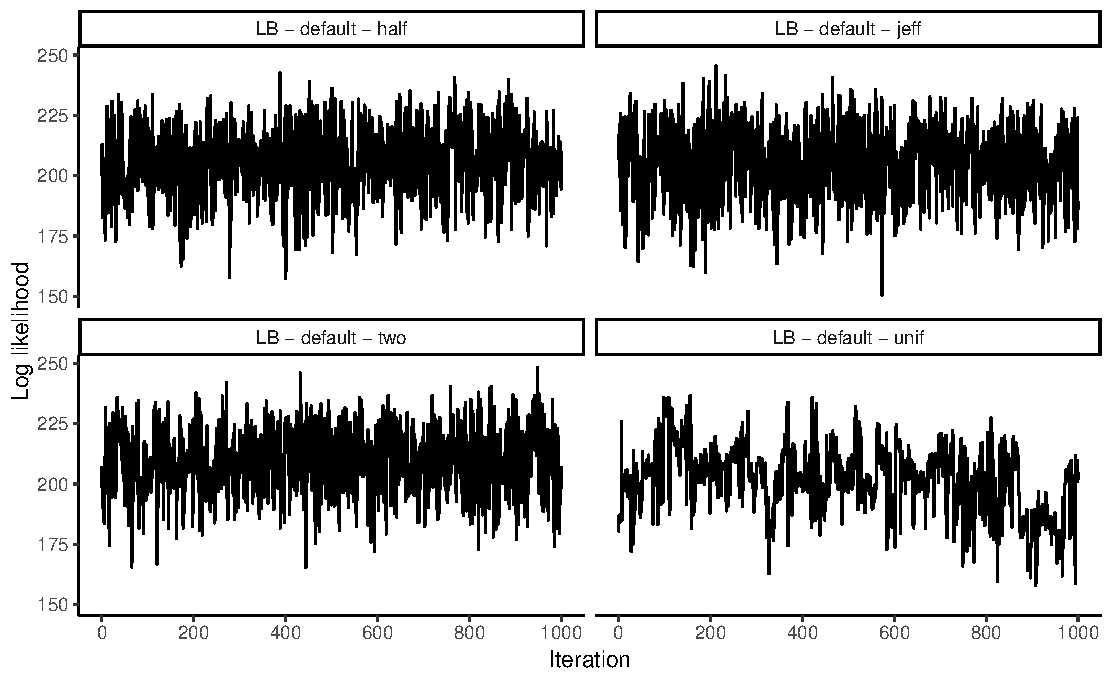
\includegraphics[width = 0.75\linewidth]{trace_case3_t_like.pdf}
	\caption{Trace plot of likelihood for case 3 (\cref{eq:synth:tau_x:case3}) with t copula. The top left denotes analysis with TBeta(0.5,0.5), top right denotes analysis with TBeta(0,0), bottom left denotes analysis with TBeta(2,2) and bottom right denotes analysis with TBeta(1,1).}
	\label{fig:case3:t:like}
\end{figure}

\begin{figure}
	\centering
	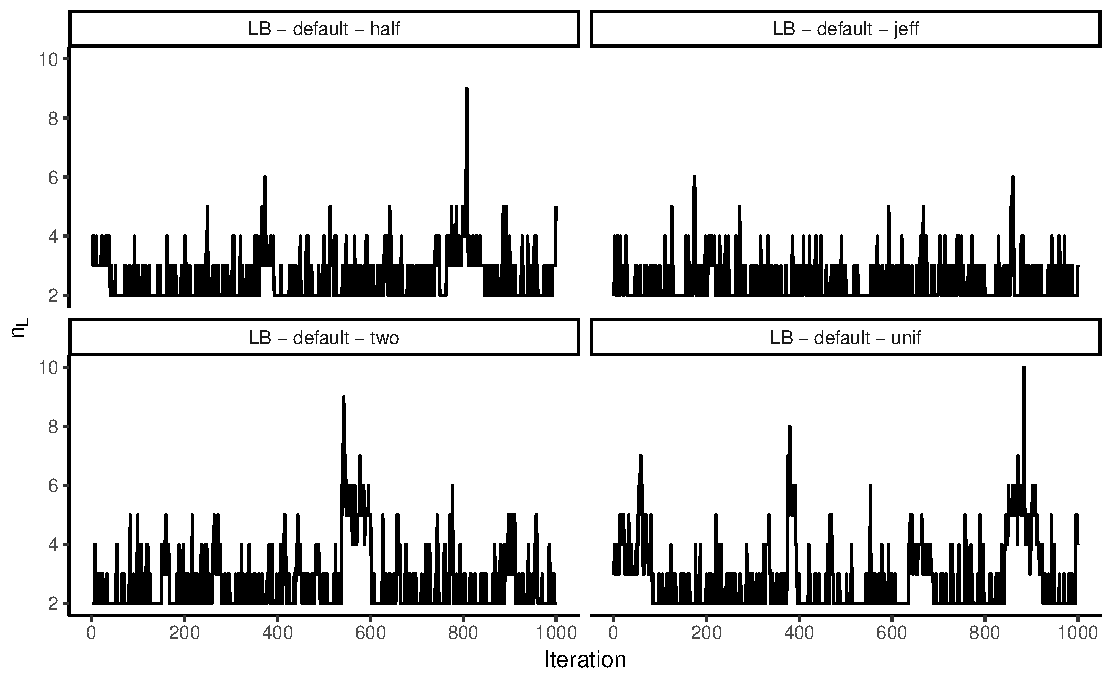
\includegraphics[width = 0.75\linewidth]{trace_case4_t_nterm.pdf}
	\caption{Trace plot of $n_L$ for case 4 (\cref{eq:synth:tau_x:case4}) with t copula. The top left denotes analysis with TBeta(0.5,0.5), top right denotes analysis with TBeta(0,0), bottom left denotes analysis with TBeta(2,2) and bottom right denotes analysis with TBeta(1,1).}
	\label{fig:case4:t:nterm}
\end{figure}

\begin{figure}
	\centering
	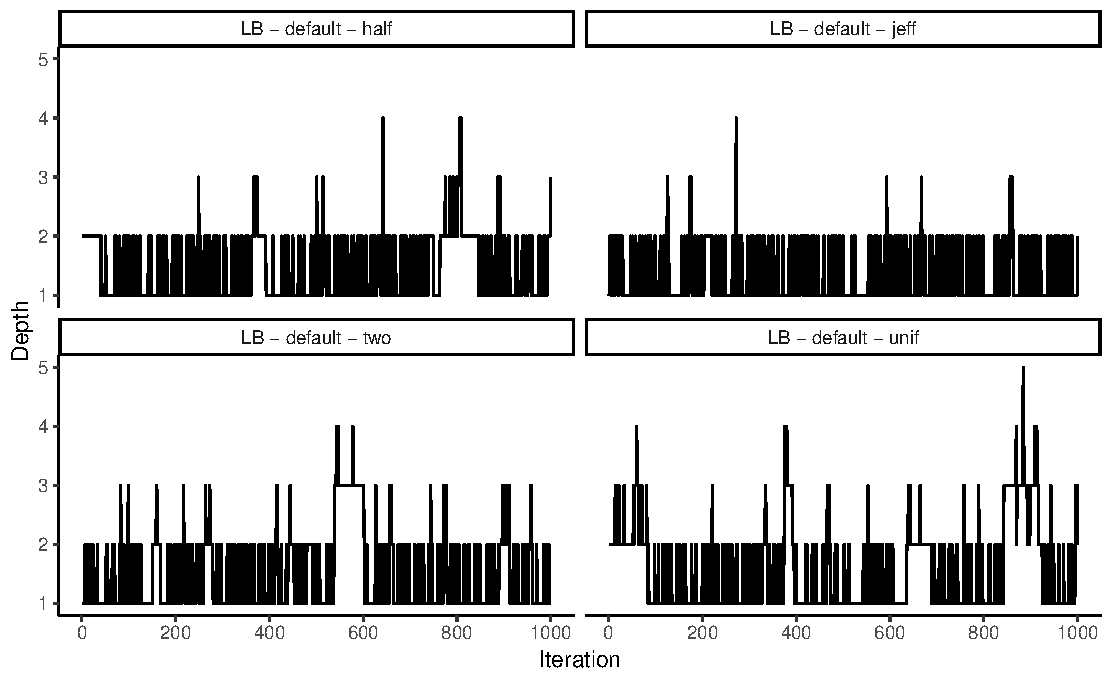
\includegraphics[width = 0.75\linewidth]{trace_case4_t_depth.pdf}
	\caption{Trace plot of depth for case 4 (\cref{eq:synth:tau_x:case4}) with t copula. The top left denotes analysis with TBeta(0.5,0.5), top right denotes analysis with TBeta(0,0), bottom left denotes analysis with TBeta(2,2) and bottom right denotes analysis with TBeta(1,1).}
	\label{fig:case4:t:depth}
\end{figure}

\begin{figure}
	\centering
	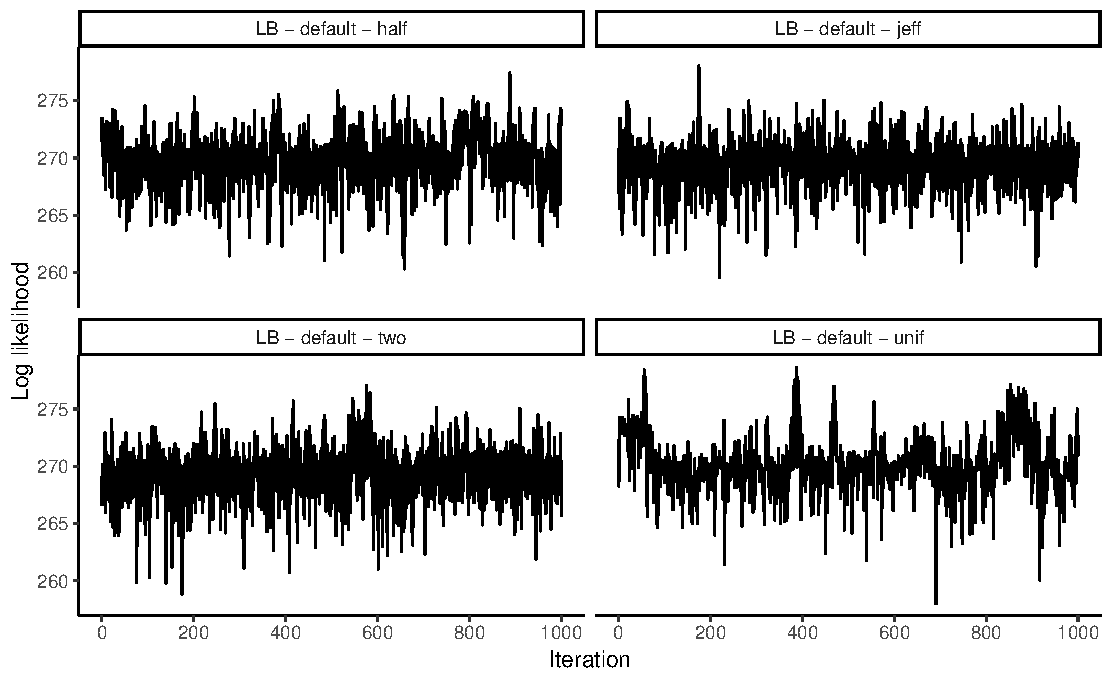
\includegraphics[width = 0.75\linewidth]{trace_case4_t_like.pdf}
	\caption{Trace plot of likelihood for case 4 (\cref{eq:synth:tau_x:case4}) with t copula. The top left denotes analysis with TBeta(0.5,0.5), top right denotes analysis with TBeta(0,0), bottom left denotes analysis with TBeta(2,2) and bottom right denotes analysis with TBeta(1,1).}
	\label{fig:case4:t:like}
\end{figure}

\subsubsection{Clayton copula} The copula parameter of the Gumbel copula lies in the open interval $(0,\infty)$. So we consider log-normal and inverse-gamma distribution for $\mu_j$

We present the summary of our analyses with Clayton copula in \cref{tab:clayton:summary}. 


\begin{table}[ht]
	\centering
	\caption{Summary of analyses with Clayton copula. The columns represents the specific case, the type of prior on $\mu_j\mid T$, the posterior expected number of terminal nodes, the posterior expected depth, the acceptance rate of MH algorithm, RMSE of estimated $\theta$ against true $\theta$, length of credible interval and coverage frequency within the credible interval. The posterior quantities are obtained by running 15000 samples in a single chain, after that we remove 5000 samples and then it is thinned by 10.}
	\label{tab:clayton:summary}
	\scriptsize{
		\begin{tabular}{ll|cccccc}
			\toprule
			& Prior on $\mu_j$ & $\mathbb{E}(n_L\mid U,X)$ & $\mathbb{E}(D\mid U,X)$ & Acc. Rate & RMSE & CI length & CI coverage \\ 
			\midrule
			Case 1 & InvGamma(1,1) & 2.867 & 1.662 & 0.232 & 0.5097 & 1.3417 & 0.764 \\ 
			(Tree) & InvGamma(2,2) & 4.246 & 2.416 & 0.300 & 0.3705 & 1.5866 & \textbf{0.924} \\ 
			& LogNorm(0,1) & 3.629 & 2.095 & 0.285 & 0.4099 & 1.5664 & 0.824 \\ 
			& LogNorm(0,5) & 3.876 & 2.178 & 0.246 & 0.3598 & 1.7381 & 0.842 \\ 
			\midrule
			Case 2 & InvGamma(1,1) & 2.291 & 1.228 & 0.202 & 0.1254 & 0.9802 & 0.880 \\ 
			(\cref{eq:synth:tau_x:case2}) & InvGamma(2,2) & 2.703 & 1.513 & 0.245 & 0.0902 & 1.2297 & \textbf{1.000} \\ 
			& LogNorm(0,1) & 2.799 & 1.581 & 0.249 & 0.0757 & 1.2844 & \textbf{1.000} \\ 
			& LogNorm(0,5) & 2.625 & 1.467 & 0.213 & 0.0834 & 1.2934 & \textbf{1.000} \\ 
			\midrule
			Case 3 & InvGamma(1,1) & 3.388 & 2.060 & 0.229 & 0.6166 & 2.2269 & 0.754 \\ 
			(\cref{eq:synth:tau_x:case3}) & InvGamma(2,2) & 3.588 & 2.125 & 0.259 & 0.5407 & 2.5436 & 0.822 \\ 
			& LogNorm(0,1) & 3.679 & 2.147 & 0.232 & 0.5492 & 2.4543 & \textbf{0.902} \\ 
			& LogNorm(0,5) & 3.516 & 2.111 & 0.265 & 0.5881 & 2.4645 & 0.884 \\ 
			\midrule
			Case 4 & InvGamma(1,1) & 2.205 & 1.183 & 0.207 & 0.0492 & 1.0143 & \textbf{0.978} \\ 
			(\cref{eq:synth:tau_x:case4}) & InvGamma(2,2) & 2.318 & 1.260 & 0.214 & 0.0527 & 1.0409 & 0.974 \\ 
			& LogNorm(0,1) & 2.377 & 1.301 & 0.241 & 0.0531 & 1.0920 & 0.972 \\ 
			& LogNorm(0,5) & 2.407 & 1.320 & 0.204 & 0.0561 & 1.1192 & 0.974 \\ 
	\end{tabular}}
\end{table}

\paragraph{Convergence Diagnostic}
\begin{table}[ht]
	\centering
	\caption{Posterior convergence diagnostic for Clayton copula. The first two columns represent the specific case, type of prior on $\mu_j\mid T$. Followed by auto-correlation (lag-1) denoted by `AC', effective sample size percentage denoted by `ESS (\%)' and Geweke score of posterior samples of depth, posterior samples of the number of terminal nodes and likelihood. To obtain the reduced samples we discard 5000 burnin samples followed by thinning of 10.}
	\scriptsize{
		\begin{tabular}{ll|crr|crr|crr}
			\toprule
		\multicolumn{2}{c|}{} &
		\multicolumn{3}{c|}{Depth} &
		\multicolumn{3}{c|}{$n_L$} &
		\multicolumn{3}{c}{likelihood} \\
		\midrule
		& Prior & AC & ESS (\%) & Geweke & AC & ESS (\%) & Geweke & AC & ESS (\%) & Geweke \\ 
			\midrule
			Case 1 & InvGamma(2,2) & 0.96 & 0.56 & 0.44 & 0.97 & 0.75 & 0.93 & 0.78 & 2.15 & -2.22 \\ 
			all sample & InvGamma(1,1) & 0.91 & 0.80 & -7.01 & 0.93 & 1.38 & -6.73 & 0.97 & 0.99 & 1.43 \\ 
			& LogNorm(0,1) & 0.95 & 0.85 & 0.31 & 0.96 & 1.05 & 1.16 & 0.83 & 1.30 & -0.90 \\ 
			& LogNorm(0,5) & 0.92 & 1.77 & 0.97 & 0.95 & 0.95 & 0.92 & 0.78 & 1.66 & 2.05 \\ 
			\midrule
			reduced sample & InvGamma(2,2) & 0.79 & 2.91 & -0.99 & 0.82 & 4.49 & -0.61 & 0.41 & 13.94 & -0.60 \\ 
			& InvGamma(1,1) & 0.64 & 7.45 & -0.14 & 0.60 & 12.20 & -0.98 & 0.84 & 4.35 & -0.50 \\ 
			& LogNorm(0,1) & 0.73 & 8.41 & 1.50 & 0.75 & 5.76 & 1.11 & 0.53 & 11.90 & -1.76 \\ 
			& LogNorm(0,5) & 0.61 & 6.01 & -2.90 & 0.69 & 3.87 & -4.00 & 0.38 & 10.90 & 1.38 \\ 
			 \midrule
			Case 2 & InvGamma(2,2) & 0.91 & 1.08 & -0.46 & 0.95 & 1.30 & -0.28 & 0.66 & 9.01 & 0.83 \\ 
			all sample & InvGamma(1,1) & 0.83 & 4.55 & -1.46 & 0.88 & 3.81 & -1.56 & 0.90 & 4.86 & -0.24 \\ 
			& LogNorm(0,1) & 0.91 & 1.14 & -1.41 & 0.94 & 1.50 & -1.55 & 0.68 & 9.35 & 1.33 \\ 
			& LogNorm(0,5) & 0.90 & 1.95 & -0.62 & 0.93 & 2.00 & -0.92 & 0.67 & 12.93 & 0.48 \\ 
			\midrule
			reduced sample & InvGamma(2,2) & 0.58 & 11.16 & 0.02 & 0.65 & 13.23 & 0.22 & 0.13 & 55.62 & -0.59 \\ 
			& InvGamma(1,1) & 0.21 & 64.79 & -2.20 & 0.33 & 50.02 & -1.70 & 0.41 & 35.19 & -0.14 \\ 
			& LogNorm(0,1) & 0.59 & 7.47 & -1.83 & 0.65 & 7.92 & -1.41 & 0.10 & 58.61 & 3.32 \\ 
			& LogNorm(0,5) & 0.57 & 14.31 & 1.14 & 0.64 & 18.75 & 0.67 & 0.13 & 64.29 & -0.84 \\ 
			\midrule
			Case 3 & InvGamma(2,2) & 0.89 & 4.39 & 0.75 & 0.92 & 3.82 & 0.63 & 0.72 & 13.42 & 1.94 \\ 
			all sample & InvGamma(1,1) & 0.97 & 0.36 & 1.70 & 0.96 & 0.49 & 2.51 & 0.97 & 1.24 & 0.49 \\ 
			& LogNorm(0,1) & 0.90 & 3.86 & -1.50 & 0.93 & 3.00 & -1.67 & 0.75 & 10.13 & 1.70 \\ 
			& LogNorm(0,5) & 0.93 & 2.50 & 4.17 & 0.94 & 2.47 & 4.81 & 0.77 & 7.87 & 0.95 \\ 
			\midrule
			reduced sample & InvGamma(2,2) & 0.32 & 51.31 & 0.86 & 0.46 & 36.65 & 0.65 & 0.14 & 75.77 & 1.55 \\ 
			& InvGamma(1,1) & 0.34 & 48.78 & -1.23 & 0.39 & 44.29 & -1.03 & 0.74 & 14.64 & -1.51 \\ 
			& LogNorm(0,1) & 0.50 & 33.42 & -0.15 & 0.58 & 26.89 & 0.33 & 0.14 & 75.50 & 0.48 \\ 
			& LogNorm(0,5) & 0.41 & 41.85 & 0.41 & 0.46 & 37.22 & 0.25 & 0.11 & 50.67 & -1.52 \\ 
			\midrule
			Case 4 & InvGamma(2,2) & 0.90 & 4.16 & -1.66 & 0.94 & 2.11 & -2.24 & 0.78 & 6.62 & 1.07 \\ 
			all sample & InvGamma(1,1) & 0.91 & 2.64 & -0.82 & 0.92 & 3.41 & 0.32 & 0.97 & 1.14 & 2.78 \\ 
			& LogNorm(0,1) & 0.89 & 4.04 & -1.43 & 0.91 & 3.45 & -1.31 & 0.76 & 10.21 & 2.55 \\ 
			& LogNorm(0,5) & 0.95 & 0.98 & 0.34 & 0.96 & 1.40 & 0.41 & 0.79 & 5.41 & 1.52 \\ 
			\midrule
			reduced sample & InvGamma(2,2) & 0.49 & 22.10 & -0.53 & 0.61 & 12.75 & -0.83 & 0.19 & 41.46 & 0.37 \\ 
			& InvGamma(1,1) & 0.36 & 44.02 & 1.31 & 0.40 & 42.72 & 0.68 & 0.74 & 14.69 & 1.07 \\ 
			& LogNorm(0,1) & 0.34 & 35.92 & 1.14 & 0.48 & 27.42 & 1.32 & 0.15 & 74.26 & 0.96 \\ 
			& LogNorm(0,5) & 0.65 & 4.46 & 19.87 & 0.69 & 5.54 & 7.37 & 0.19 & 43.53 & -3.11 \\ 
			\bottomrule
	\end{tabular}}
\end{table}


\paragraph{Trace-plots} We present trace-plots for $n_l$, depth and likelihood for case 1 in \cref{fig:case1:clayton:nterm,fig:case1:clayton:depth,fig:case1:clayton:like}. Similarly for case 2 the trace-plots are provided in \cref{fig:case2:clayton:nterm,fig:case2:clayton:depth,fig:case2:clayton:like}; for case 3 the trace-plots are provided in \cref{fig:case3:clayton:nterm,fig:case3:clayton:depth,fig:case3:clayton:like}; and for case 4 the trace-plots are provided in \cref{fig:case4:clayton:nterm,fig:case4:clayton:depth,fig:case4:clayton:like}.

% LogNorm(0,1) seems nice, acceptance rate is over-all better than others and likelihood seems more consistent

\begin{figure}
	\centering
	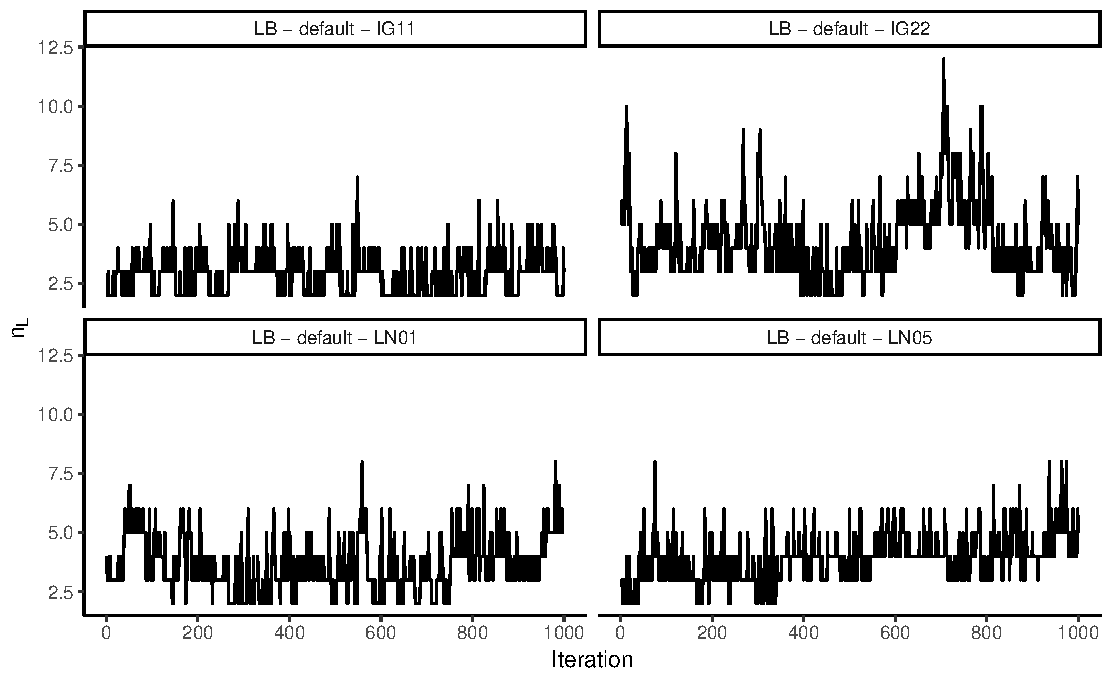
\includegraphics[width = 0.75\linewidth]{trace_case1_clayton_nterm.pdf}
	\caption{Trace plot of $n_L$ for case 1 (tree structure) with Clayton copula. The top left denotes analysis with InvInvGamma(1,1), top right denotes analysis with InvInvGamma(2,2), bottom left denotes analysis with LogNormal(0,1) and bottom right denotes analysis with LogNormal(0,5).}
	\label{fig:case1:clayton:nterm}
\end{figure}

\begin{figure}
	\centering
	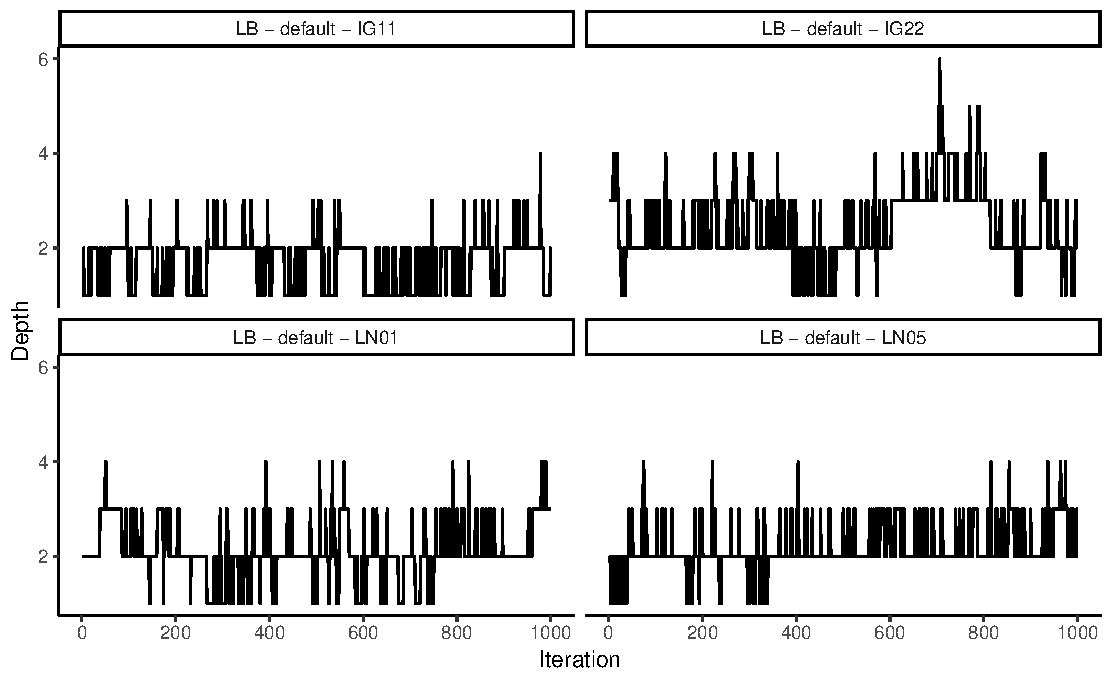
\includegraphics[width = 0.75\linewidth]{trace_case1_clayton_depth.pdf}
	\caption{Trace plot of depth for case 1 (tree structure) with Clayton copula. The top left denotes analysis with InvInvGamma(1,1), top right denotes analysis with InvInvGamma(2,2), bottom left denotes analysis with LogNormal(0,1) and bottom right denotes analysis with LogNormal(0,5).}
	\label{fig:case1:clayton:depth}
\end{figure}

\begin{figure}
	\centering
	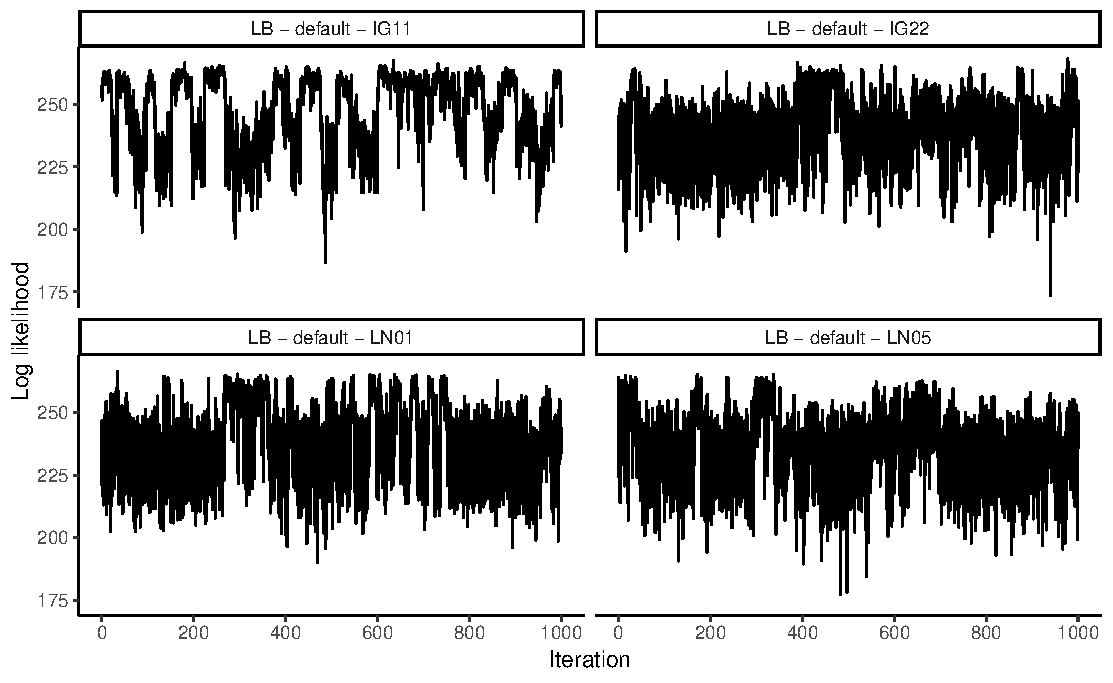
\includegraphics[width = 0.75\linewidth]{trace_case1_clayton_like.pdf}
	\caption{Trace plot of likelihood for case 1 (tree structure) with Clayton copula. The top left denotes analysis with InvInvGamma(1,1), top right denotes analysis with InvInvGamma(2,2), bottom left denotes analysis with LogNormal(0,1) and bottom right denotes analysis with LogNormal(0,5).}
	\label{fig:case1:clayton:like}
\end{figure}

\begin{figure}
	\centering
	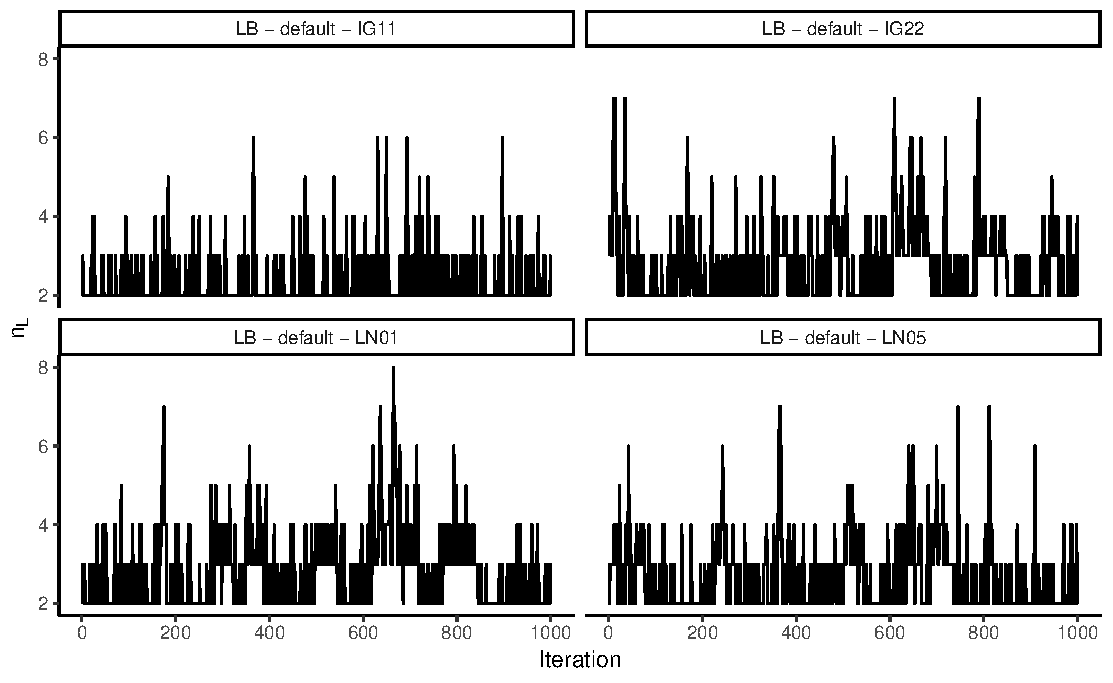
\includegraphics[width = 0.75\linewidth]{trace_case2_clayton_nterm.pdf}
	\caption{Trace plot of $n_L$ for case 2 (\cref{eq:synth:tau_x:case2}) with Clayton copula. The top left denotes analysis with InvInvGamma(1,1), top right denotes analysis with InvInvGamma(2,2), bottom left denotes analysis with LogNormal(0,1) and bottom right denotes analysis with LogNormal(0,5).}
	\label{fig:case2:clayton:nterm}
\end{figure}

\begin{figure}
	\centering
	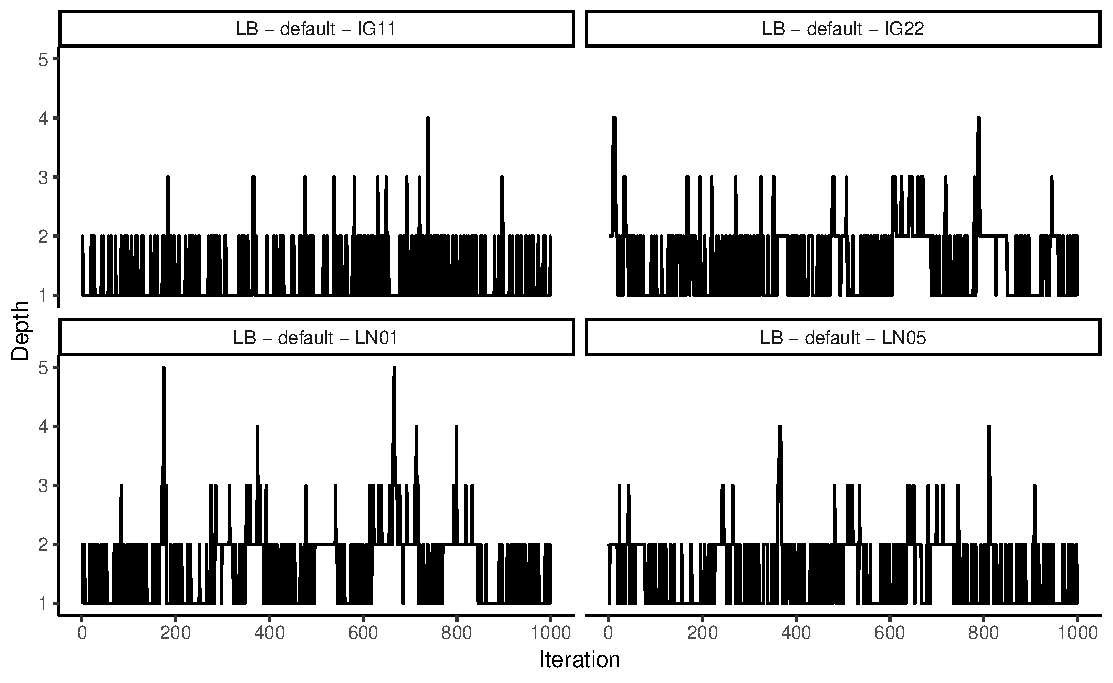
\includegraphics[width = 0.75\linewidth]{trace_case2_clayton_depth.pdf}
	\caption{Trace plot of depth for case 2 (\cref{eq:synth:tau_x:case2}) with Clayton copula. The top left denotes analysis with InvInvGamma(1,1), top right denotes analysis with InvInvGamma(2,2), bottom left denotes analysis with LogNormal(0,1) and bottom right denotes analysis with LogNormal(0,5).}
	\label{fig:case2:clayton:depth}
\end{figure}

\begin{figure}
	\centering
	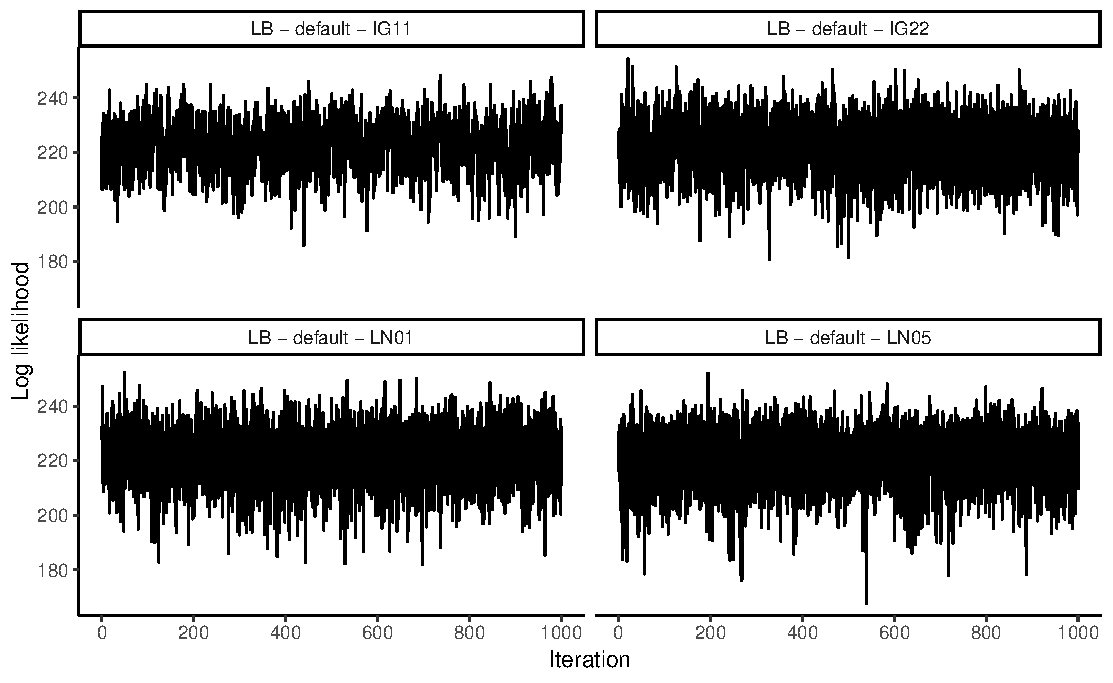
\includegraphics[width = 0.75\linewidth]{trace_case2_clayton_like.pdf}
	\caption{Trace plot of likelihood for case 2 (\cref{eq:synth:tau_x:case2}) with Clayton copula. The top left denotes analysis with InvInvGamma(1,1), top right denotes analysis with InvInvGamma(2,2), bottom left denotes analysis with LogNormal(0,1) and bottom right denotes analysis with LogNormal(0,5).}
	\label{fig:case2:clayton:like}
\end{figure}

\begin{figure}
	\centering
	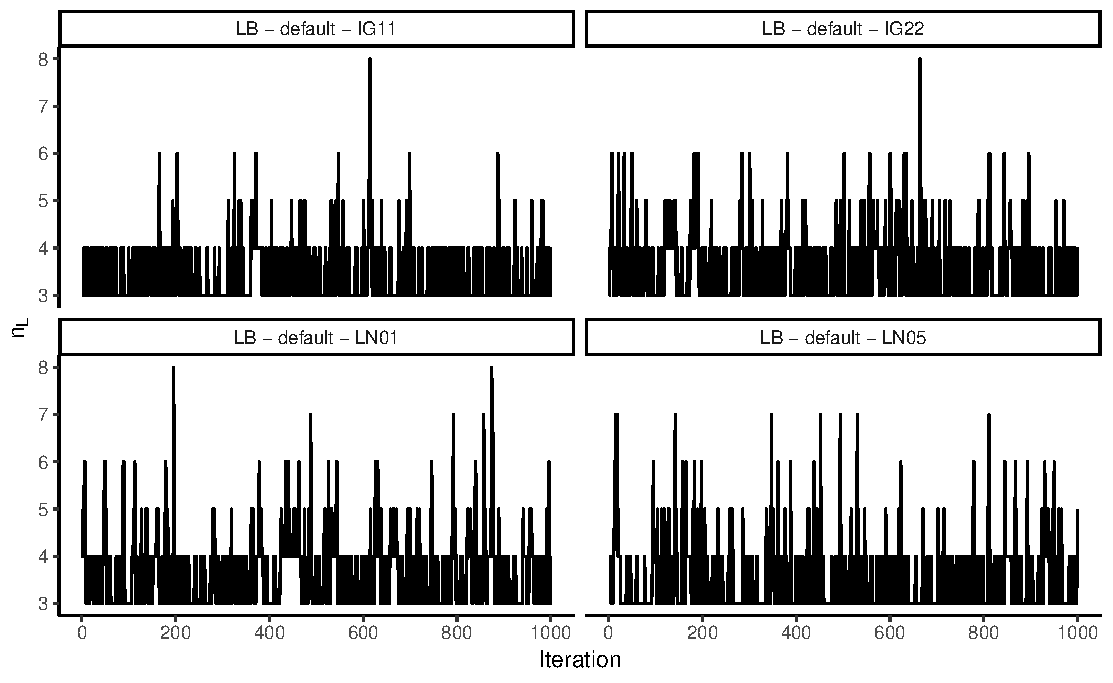
\includegraphics[width = 0.75\linewidth]{trace_case3_clayton_nterm.pdf}
	\caption{Trace plot of $n_L$ for case 3 (\cref{eq:synth:tau_x:case3}) with Clayton copula. The top left denotes analysis with InvInvGamma(1,1), top right denotes analysis with InvInvGamma(2,2), bottom left denotes analysis with LogNormal(0,1) and bottom right denotes analysis with LogNormal(0,5).}
	\label{fig:case3:clayton:nterm}
\end{figure}

\begin{figure}
	\centering
	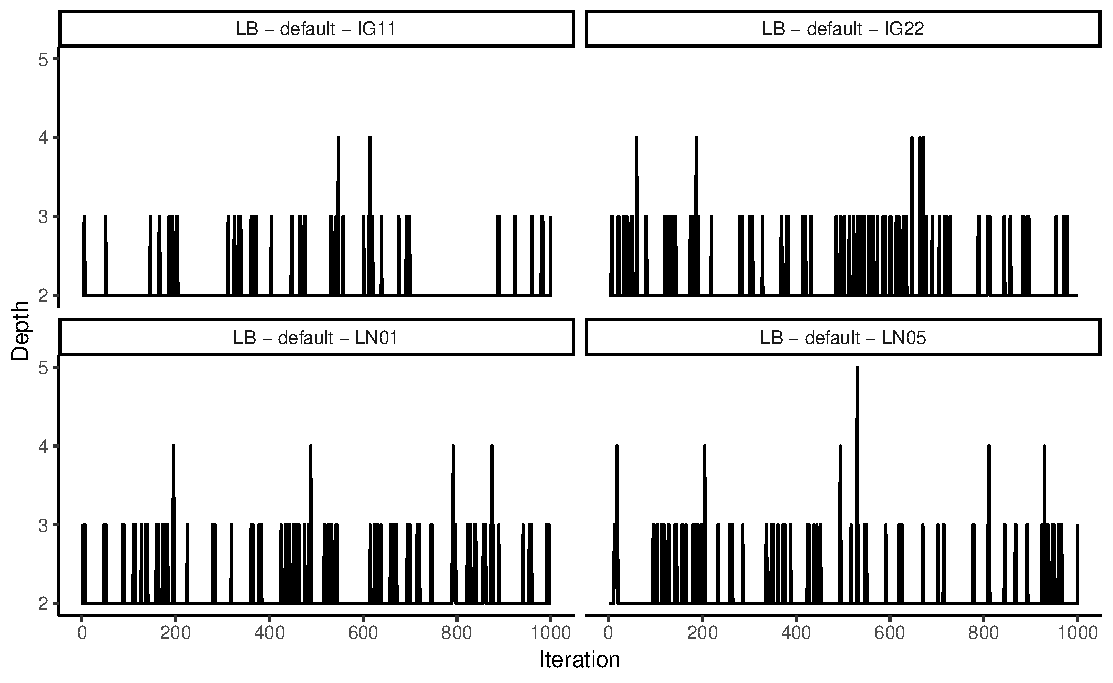
\includegraphics[width = 0.75\linewidth]{trace_case3_clayton_depth.pdf}
	\caption{Trace plot of depth for case 3 (\cref{eq:synth:tau_x:case3}) with Clayton copula. The top left denotes analysis with InvInvGamma(1,1), top right denotes analysis with InvInvGamma(2,2), bottom left denotes analysis with LogNormal(0,1) and bottom right denotes analysis with LogNormal(0,5).}
	\label{fig:case3:clayton:depth}
\end{figure}

\begin{figure}
	\centering
	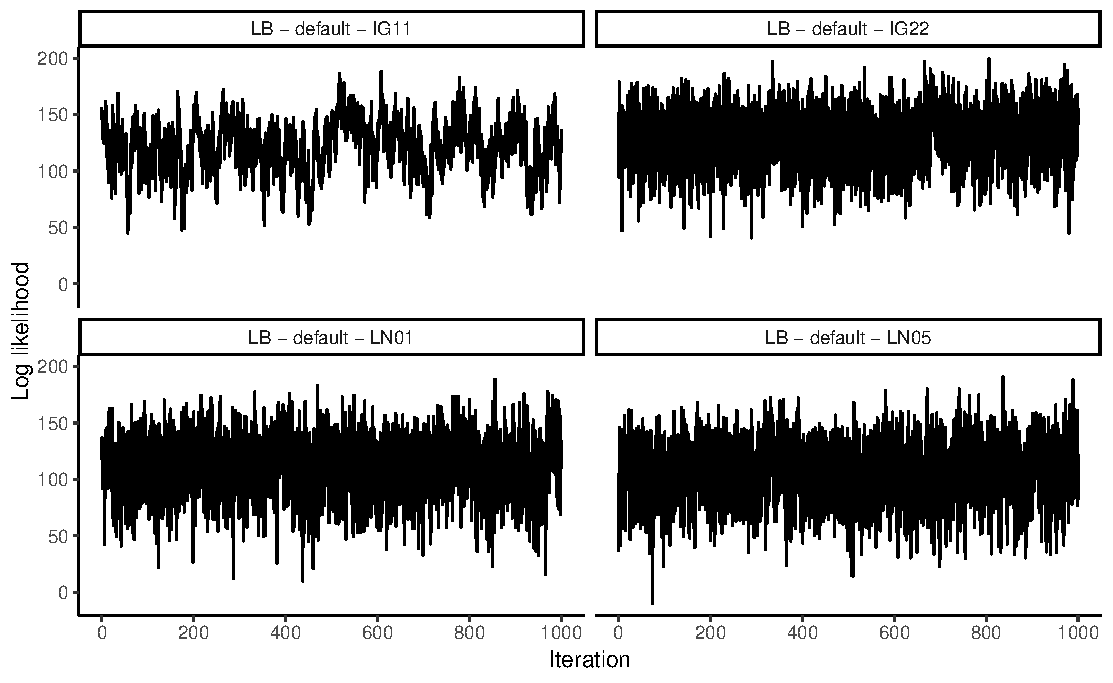
\includegraphics[width = 0.75\linewidth]{trace_case3_clayton_like.pdf}
	\caption{Trace plot of likelihood for case 3 (\cref{eq:synth:tau_x:case3}) with Clayton copula. The top left denotes analysis with InvInvGamma(1,1), top right denotes analysis with InvInvGamma(2,2), bottom left denotes analysis with LogNormal(0,1) and bottom right denotes analysis with LogNormal(0,5).}
	\label{fig:case3:clayton:like}
\end{figure}

\begin{figure}
	\centering
	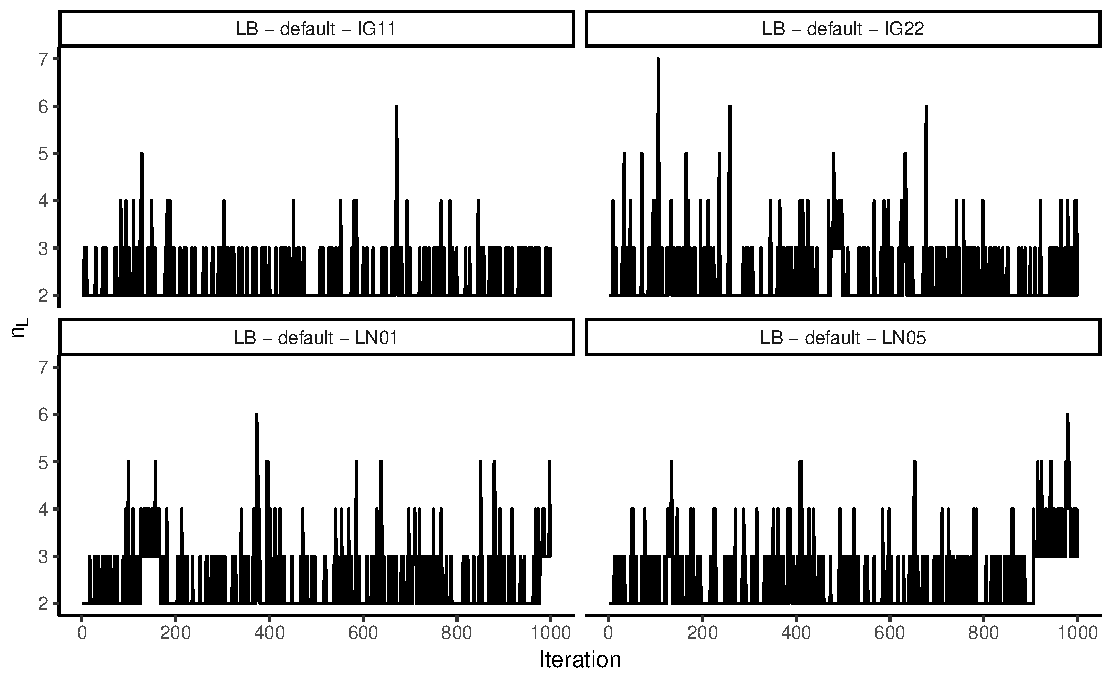
\includegraphics[width = 0.75\linewidth]{trace_case4_clayton_nterm.pdf}
	\caption{Trace plot of $n_L$ for case 4 (\cref{eq:synth:tau_x:case4}) with Clayton copula. The top left denotes analysis with InvInvGamma(1,1), top right denotes analysis with InvInvGamma(2,2), bottom left denotes analysis with LogNormal(0,1) and bottom right denotes analysis with LogNormal(0,5).}
	\label{fig:case4:clayton:nterm}
\end{figure}

\begin{figure}
	\centering
	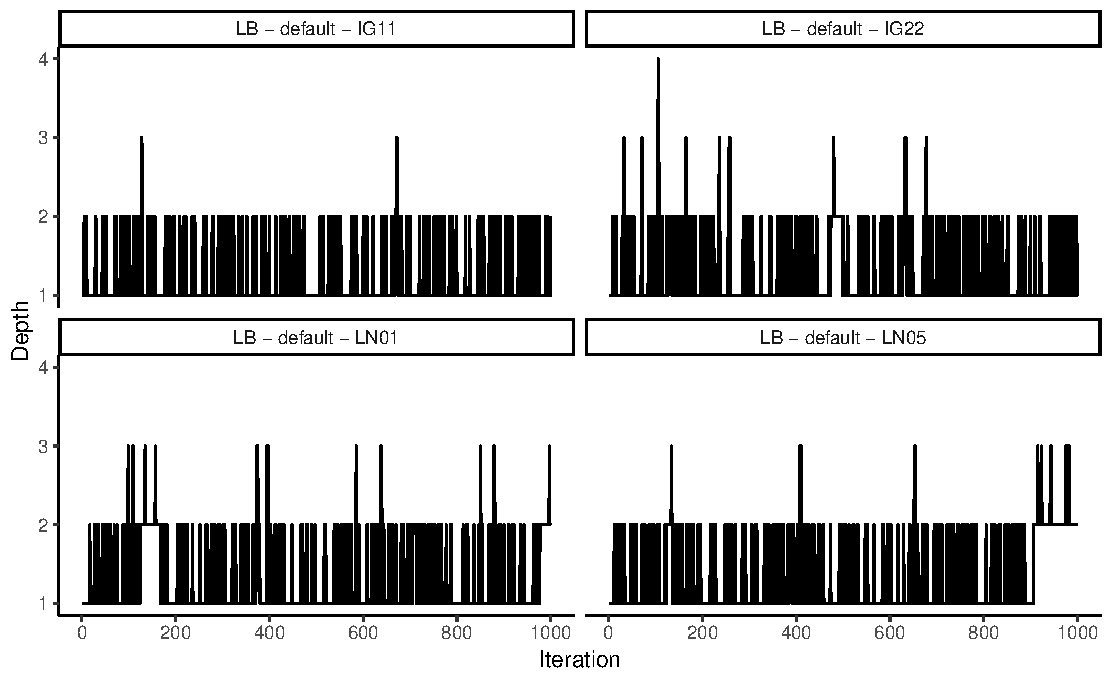
\includegraphics[width = 0.75\linewidth]{trace_case4_clayton_depth.pdf}
	\caption{Trace plot of depth for case 4 (\cref{eq:synth:tau_x:case4}) with Clayton copula. The top left denotes analysis with InvInvGamma(1,1), top right denotes analysis with InvInvGamma(2,2), bottom left denotes analysis with LogNormal(0,1) and bottom right denotes analysis with LogNormal(0,5).}
	\label{fig:case4:clayton:depth}
\end{figure}

\begin{figure}
	\centering
	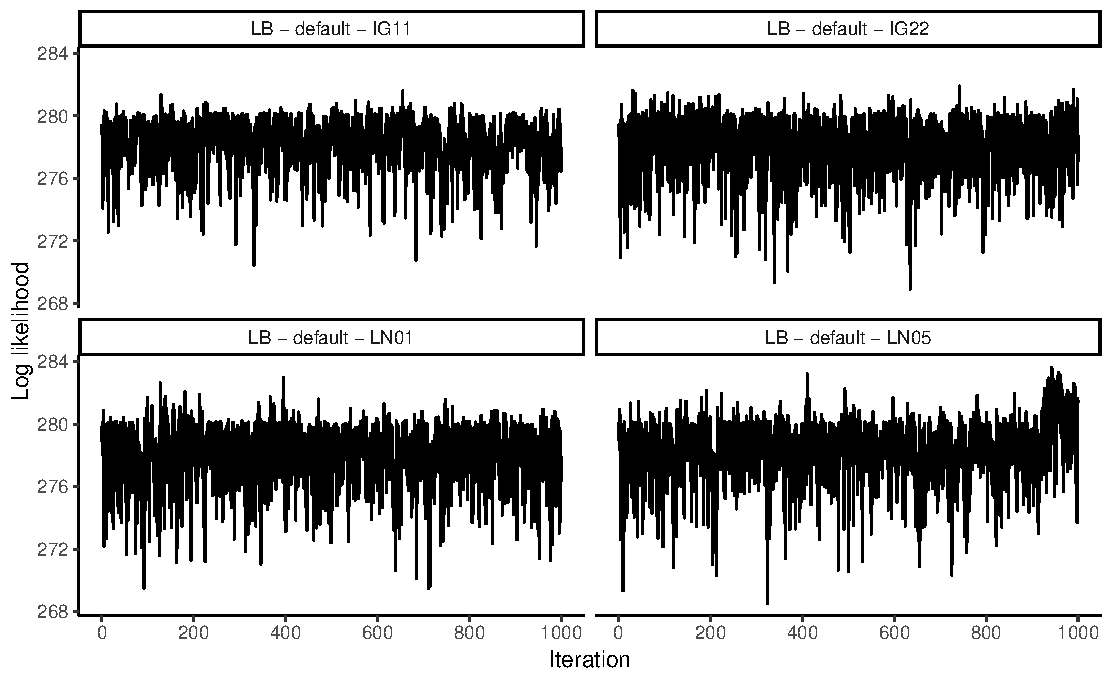
\includegraphics[width = 0.75\linewidth]{trace_case4_clayton_like.pdf}
	\caption{Trace plot of likelihood for case 4 (\cref{eq:synth:tau_x:case4}) with Clayton copula. The top left denotes analysis with InvInvGamma(1,1), top right denotes analysis with InvInvGamma(2,2), bottom left denotes analysis with LogNormal(0,1) and bottom right denotes analysis with LogNormal(0,5).}
	\label{fig:case4:clayton:like}
\end{figure}

\subsubsection{Gumbel copula} The copula parameter of the Gumbel copula lies in the open interval $[1,\infty)$. So we consider log-normal and inverse-gamma distribution for $\mu_j$.

We present the summary of our analyses with Gumbel copula in \cref{tab:gumbel:summary}. 


\begin{table}[ht]
	\centering
	\caption{Summary of analyses with Gumbel copula. The columns represents the specific case, the type of prior on $\mu_j\mid T$, the posterior expected number of terminal nodes, the posterior expected depth, the acceptance rate of MH algorithm, RMSE of estimated $\theta$ against true $\theta$, length of credible interval and coverage frequency within the credible interval. The posterior quantities are obtained by running 15000 samples in a single chain, after that we remove 5000 samples and then it is thinned by 10.}
	\label{tab:gumbel:summary}
	\scriptsize{
	\begin{tabular}{ll|cccccc}
		\toprule
		& Prior on $\mu_j$ & $\mathbb{E}(n_L\mid U,X)$ & $\mathbb{E}(D\mid U,X)$ & Acc. Rate & RMSE & CI length & CI coverage \\ 
		\midrule
		Case 1 & InvGamma(1,1) & 4.513 & 2.397 & 0.246 & 0.1292 & 0.9088 & 0.908 \\ 
		(Tree) & InvGamma(2,2) & 4.714 & 2.532 & 0.256 & 0.1407 & 0.8179 & 0.858 \\ 
		& LogNorm(0,1) & 4.626 & 2.525 & 0.260 & 0.1321 & 0.9956 & \textbf{0.916} \\ 
		& LogNorm(0,5) & 4.389 & 2.335 & 0.227 & 0.1353 & 0.8653 & 0.856 \\ 
		\midrule
		Case 2 & InvGamma(1,1) & 2.373 & 1.289 & 0.202 & 0.0277 & 0.6032 & 0.998 \\ 
		(\cref{eq:synth:tau_x:case2}) & InvGamma(2,2) & 2.605 & 1.455 & 0.209 & 0.0262 & 0.6956 & \textbf{1.000} \\ 
		& LogNorm(0,1) & 2.349 & 1.268 & 0.214 & 0.0273 & 0.6049 & 0.994 \\ 
		& LogNorm(0,5) & 2.408 & 1.314 & 0.212 & 0.0277 & 0.6025 & 0.974 \\ 
		\midrule
		Case 3 & InvGamma(1,1) & 3.421 & 2.086 & 0.241 & 0.1523 & 1.1744 & 0.764 \\ 
		(\cref{eq:synth:tau_x:case3}) & InvGamma(2,2) & 3.429 & 2.077 & 0.252 & 0.1509 & 1.2093 & 0.788 \\ 
		& LogNorm(0,1) & 3.631 & 2.173 & 0.267 & 0.1566 & 1.1954 & 0.792 \\ 
		& LogNorm(0,5) & 3.590 & 2.119 & 0.262 & 0.1575 & 1.2772 & \textbf{0.854} \\ 
		\midrule
		Case 4 & InvGamma(1,1) & 2.706 & 1.517 & 0.247 & 0.0152 & 0.7585 & 0.974 \\ 
		(\cref{eq:synth:tau_x:case4}) & InvGamma(2,2) & 2.602 & 1.466 & 0.252 & 0.0140 & 0.7451 & 0.974 \\ 
		& LogNorm(0,1) & 2.527 & 1.405 & 0.224 & 0.0161 & 0.7377 & 0.988 \\ 
		& LogNorm(0,5) & 2.445 & 1.353 & 0.217 & 0.0148 & 0.7090 & \textbf{0.990} \\ 
		\end{tabular}}
\end{table}

\paragraph{Convergence Diagnostic}
\begin{table}[ht]
	\centering
	\caption{Posterior convergence diagnostic for Gumbel copula. The first two columns represent the specific case, type of prior on $\mu_j\mid T$. Followed by auto-correlation (lag-1) denoted by `AC', effective sample size percentage denoted by `ESS (\%)' and Geweke score of posterior samples of depth, posterior samples of the number of terminal nodes and likelihood. To obtain the reduced samples we discard 5000 burnin samples followed by thinning of 10.}
	\scriptsize{
		\begin{tabular}{ll|crr|crr|crr}
			\toprule
		\multicolumn{2}{c|}{} &
		\multicolumn{3}{c|}{Depth} &
		\multicolumn{3}{c|}{$n_L$} &
		\multicolumn{3}{c}{likelihood} \\
		\midrule
		& Prior & AC & ESS (\%) & Geweke & AC & ESS (\%) & Geweke & AC & ESS (\%) & Geweke \\ 
			\midrule
			Case 1 & InvGamma(2,2) & 0.88 & 1.40 & 13.28 & 0.93 & 1.35 & 9.66 & 0.86 & 1.62 & 8.23 \\ 
			all sample & InvGamma(1,1) & 0.90 & 1.59 & 14.60 & 0.93 & 2.01 & 9.80 & 0.87 & 1.91 & 10.05 \\ 
			& LogNorm(0,1) & 0.87 & 1.48 & 2.69 & 0.92 & 1.76 & 2.34 & 0.86 & 2.76 & 2.53 \\ 
			& LogNorm(0,5) & 0.85 & 2.40 & -1.80 & 0.89 & 2.52 & -1.21 & 0.85 & 2.57 & -0.59 \\ 
			\midrule
			reduced sample & InvGamma(2,2) & 0.32 & 47.94 & -0.64 & 0.43 & 25.79 & -0.78 & 0.36 & 44.19 & -0.17 \\ 
			& InvGamma(1,1) & 0.30 & 43.42 & -0.84 & 0.41 & 41.76 & -0.94 & 0.37 & 45.81 & -1.31 \\ 
			& LogNorm(0,1) & 0.57 & 15.31 & 1.26 & 0.63 & 12.33 & 0.97 & 0.47 & 22.66 & 0.90 \\ 
			& LogNorm(0,5) & 0.49 & 13.55 & -2.88 & 0.52 & 16.06 & -3.28 & 0.45 & 7.66 & -0.98 \\ 
			\midrule
			Case 2 & InvGamma(2,2) & 0.91 & 0.92 & -2.79 & 0.94 & 0.97 & -2.81 & 0.78 & 2.63 & 0.19 \\ 
			all sample & InvGamma(1,1) & 0.87 & 2.37 & -3.44 & 0.92 & 2.19 & -3.25 & 0.71 & 17.15 & -1.64 \\ 
			& LogNorm(0,1) & 0.84 & 3.05 & -3.12 & 0.90 & 3.21 & -3.20 & 0.71 & 16.91 & -1.39 \\ 
			& LogNorm(0,5) & 0.87 & 2.95 & -4.08 & 0.92 & 2.03 & -3.65 & 0.71 & 17.24 & 0.01 \\ 
			\midrule
			reduced sample & InvGamma(2,2) & 0.31 & 52.92 & 0.81 & 0.36 & 46.93 & 0.65 & \textbf{0.05} & 100.00 & -1.27 \\ 
			& InvGamma(1,1) & 0.55 & 9.81 & -1.63 & 0.68 & 8.82 & -2.29 & \textbf{0.06} & 100.00 & -0.86 \\ 
			& LogNorm(0,1) & 0.53 & 16.09 & -0.71 & 0.58 & 18.85 & -1.21 & 0.07 & 70.10 & -0.45 \\ 
			& LogNorm(0,5) & 0.49 & 13.28 & -0.26 & 0.55 & 13.05 & -0.16 & \textbf{0.03} & 100.00 & 1.29 \\ 
			\midrule
			Case 3 & InvGamma(2,2) & 0.86 & 6.21 & 1.15 & 0.89 & 5.27 & 1.06 & 0.68 & 7.15 & -0.25 \\ 
			all sample & InvGamma(1,1) & 0.86 & 6.80 & 1.50 & 0.90 & 5.45 & 1.08 & 0.66 & 8.14 & 1.84 \\ 
			& LogNorm(0,1) & 0.94 & 1.81 & -0.90 & 0.95 & 1.84 & -1.16 & 0.68 & 10.78 & -0.29 \\ 
			& LogNorm(0,5) & 0.89 & 4.91 & 1.09 & 0.92 & 2.62 & 1.94 & 0.70 & 7.57 & -2.84 \\ 
			\midrule
			reduced sample & InvGamma(2,2) & 0.14 & 58.08 & -1.26 & 0.26 & 58.21 & -3.38 & 0.10 & 22.12 & 1.92 \\ 
			& InvGamma(1,1) & 0.20 & 49.04 & -1.79 & 0.31 & 52.44 & -0.05 & 0.14 & 65.67 & 0.53 \\ 
			& LogNorm(0,1) & 0.54 & 20.23 & 1.12 & 0.53 & 25.72 & 0.89 & 0.15 & 62.36 & -1.08 \\ 
			& LogNorm(0,5) & 0.46 & 35.09 & 1.01 & 0.47 & 30.96 & 1.71 & 0.11 & 40.65 & 1.21 \\ 
			\midrule
			Case 4 & InvGamma(2,2) & 0.93 & 1.66 & 0.10 & 0.95 & 1.86 & 0.06 & 0.72 & 4.10 & -0.21 \\ 
			all sample & InvGamma(1,1) & 0.91 & 3.58 & 1.00 & 0.94 & 2.69 & 0.02 & 0.75 & 4.80 & -0.70 \\ 
			& LogNorm(0,1) & 0.89 & 4.14 & -0.04 & 0.92 & 3.53 & 1.06 & 0.71 & 6.72 & 0.22 \\ 
			& LogNorm(0,5) & 0.90 & 4.18 & 0.69 & 0.93 & 3.24 & 0.53 & 0.84 & 0.76 & 1.17 \\ 
			\midrule
			reduced sample & InvGamma(2,2) & 0.71 & 13.53 & -0.32 & 0.70 & 11.16 & -0.05 & 0.26 & 31.32 & -0.78 \\ 
			& InvGamma(1,1) & 0.46 & 31.79 & -0.08 & 0.57 & 27.62 & -0.31 & 0.30 & 20.51 & 0.17 \\ 
			& LogNorm(0,1) & 0.28 & 57.84 & 1.54 & 0.40 & 38.27 & 1.73 & 0.24 & 27.89 & 0.66 \\ 
			& LogNorm(0,5) & 0.45 & 37.97 & -0.40 & 0.49 & 33.99 & -1.06 & 0.63 & 3.14 & 0.74 \\ 
			\bottomrule
	\end{tabular}}
\end{table}

\paragraph{Trace-plots} We present trace-plots for $n_l$, depth and likelihood for case 1 in \cref{fig:case1:gumbel:nterm,fig:case1:gumbel:depth,fig:case1:gumbel:like}. Similarly for case 2 the trace-plots are provided in \cref{fig:case2:gumbel:nterm,fig:case2:gumbel:depth,fig:case2:gumbel:like}; for case 3 the trace-plots are provided in \cref{fig:case3:gumbel:nterm,fig:case3:gumbel:depth,fig:case3:gumbel:like}; and for case 4 the trace-plots are provided in \cref{fig:case4:gumbel:nterm,fig:case4:gumbel:depth,fig:case4:gumbel:like}.

% LogNorm(0,1) seems nice, acceptance rate is over-all better than others and likelihood seems more consistent

\begin{figure}
	\centering
	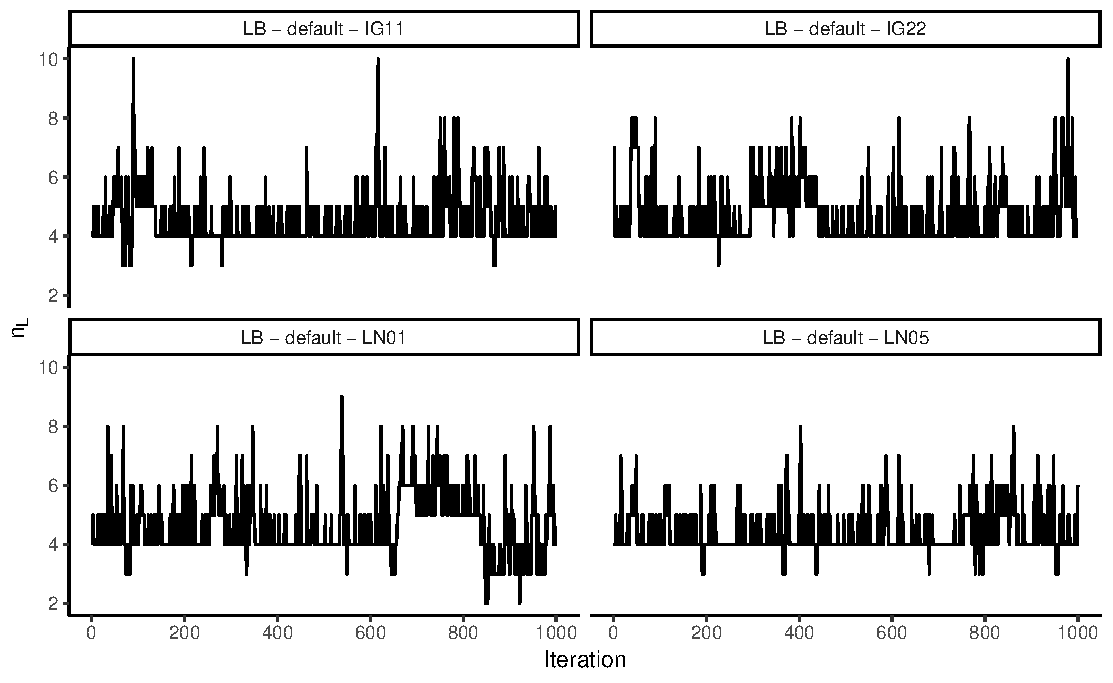
\includegraphics[width = 0.75\linewidth]{trace_case1_gumbel_nterm.pdf}
	\caption{Trace plot of $n_L$ for case 1 (tree structure) with Gumbel copula. The top left denotes analysis with InvInvGamma(1,1), top right denotes analysis with InvInvGamma(2,2), bottom left denotes analysis with LogNormal(0,1) and bottom right denotes analysis with LogNormal(0,5).}
	\label{fig:case1:gumbel:nterm}
\end{figure}

\begin{figure}
	\centering
	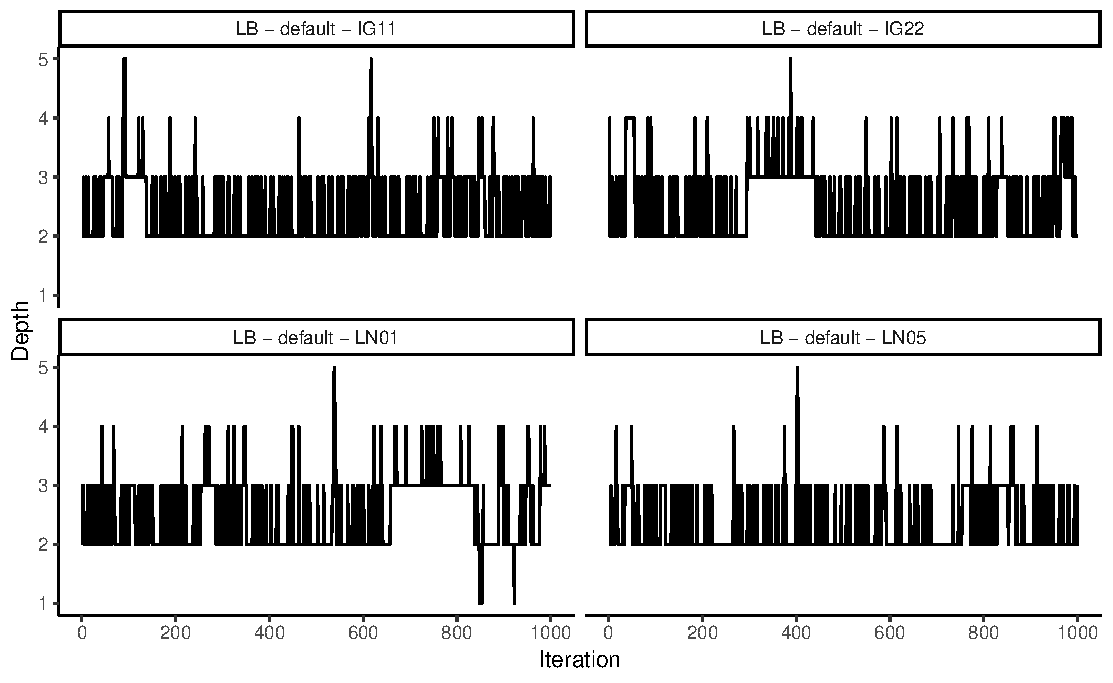
\includegraphics[width = 0.75\linewidth]{trace_case1_gumbel_depth.pdf}
	\caption{Trace plot of depth for case 1 (tree structure) with Gumbel copula. The top left denotes analysis with InvInvGamma(1,1), top right denotes analysis with InvInvGamma(2,2), bottom left denotes analysis with LogNormal(0,1) and bottom right denotes analysis with LogNormal(0,5).}
	\label{fig:case1:gumbel:depth}
\end{figure}

\begin{figure}
	\centering
	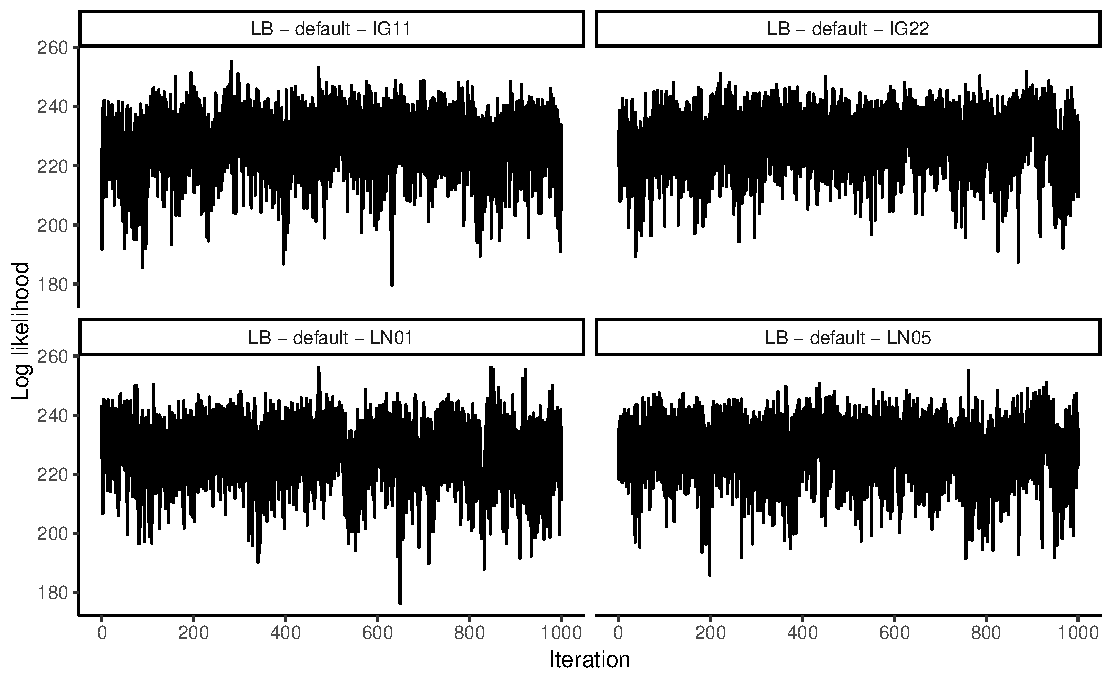
\includegraphics[width = 0.75\linewidth]{trace_case1_gumbel_like.pdf}
	\caption{Trace plot of likelihood for case 1 (tree structure) with Gumbel copula. The top left denotes analysis with InvInvGamma(1,1), top right denotes analysis with InvInvGamma(2,2), bottom left denotes analysis with LogNormal(0,1) and bottom right denotes analysis with LogNormal(0,5).}
	\label{fig:case1:gumbel:like}
\end{figure}

\begin{figure}
	\centering
	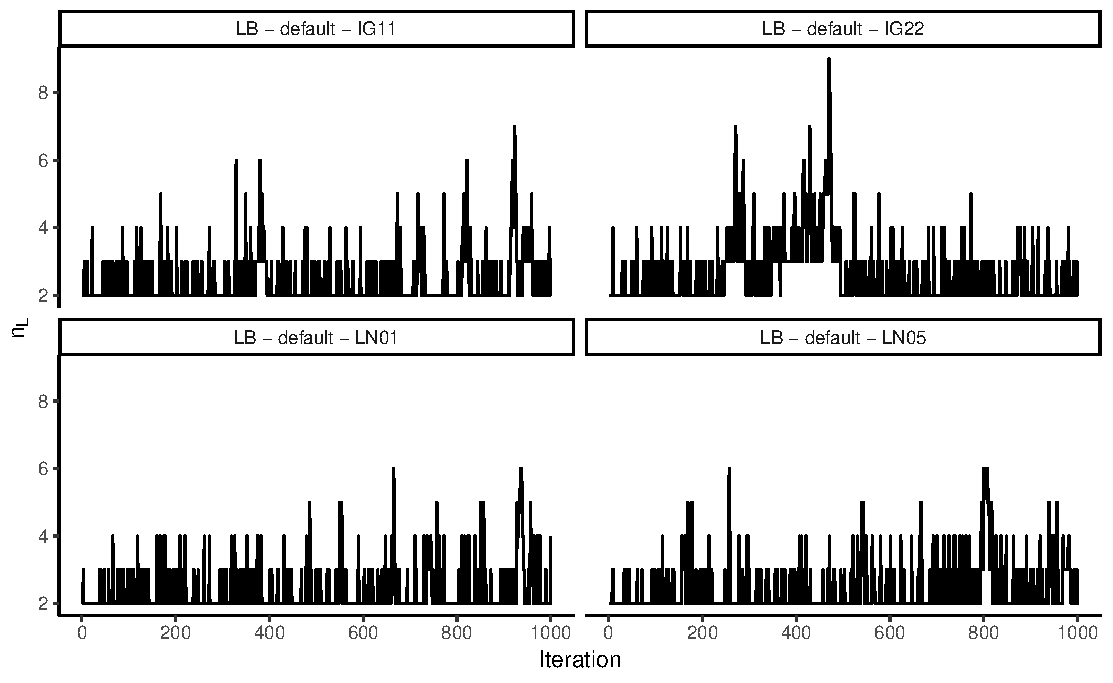
\includegraphics[width = 0.75\linewidth]{trace_case2_gumbel_nterm.pdf}
	\caption{Trace plot of $n_L$ for case 2 (\cref{eq:synth:tau_x:case2}) with Gumbel copula. The top left denotes analysis with InvInvGamma(1,1), top right denotes analysis with InvInvGamma(2,2), bottom left denotes analysis with LogNormal(0,1) and bottom right denotes analysis with LogNormal(0,5).}
	\label{fig:case2:gumbel:nterm}
\end{figure}

\begin{figure}
	\centering
	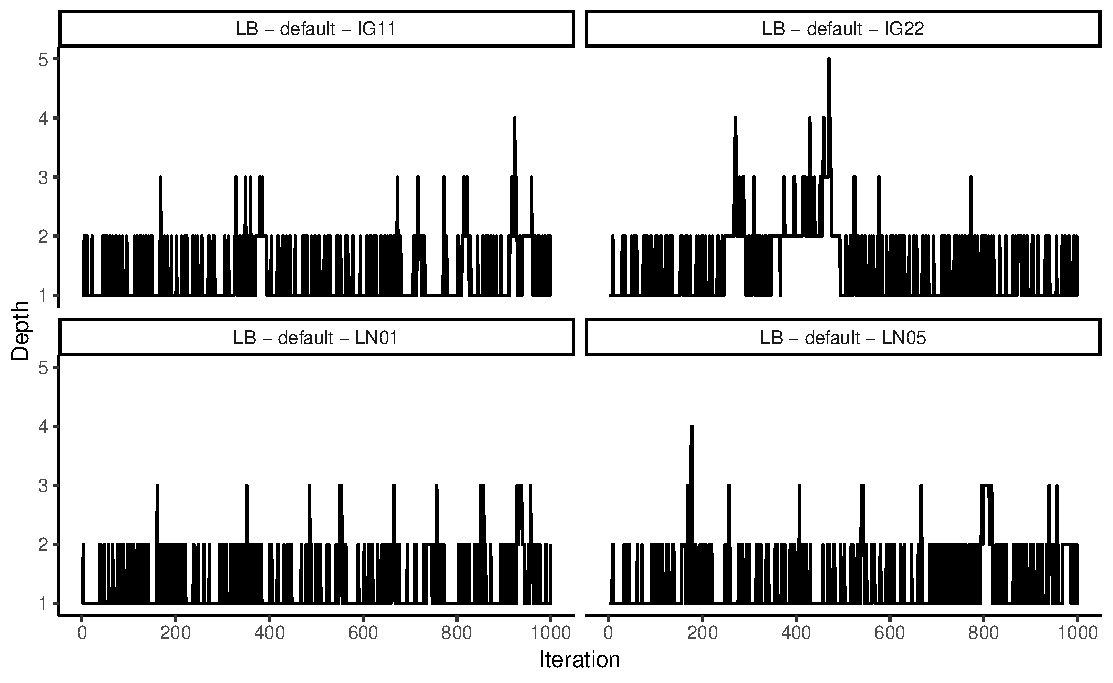
\includegraphics[width = 0.75\linewidth]{trace_case2_gumbel_depth.pdf}
	\caption{Trace plot of depth for case 2 (\cref{eq:synth:tau_x:case2}) with Gumbel copula. The top left denotes analysis with InvInvGamma(1,1), top right denotes analysis with InvInvGamma(2,2), bottom left denotes analysis with LogNormal(0,1) and bottom right denotes analysis with LogNormal(0,5).}
	\label{fig:case2:gumbel:depth}
\end{figure}

\begin{figure}
	\centering
	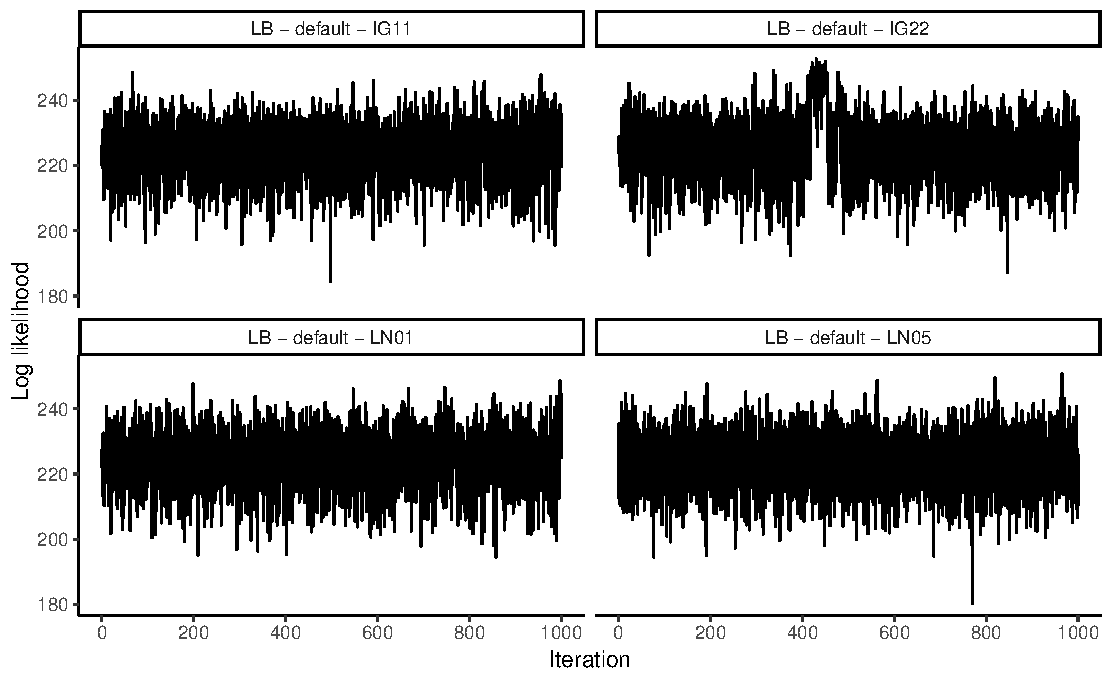
\includegraphics[width = 0.75\linewidth]{trace_case2_gumbel_like.pdf}
	\caption{Trace plot of likelihood for case 2 (\cref{eq:synth:tau_x:case2}) with Gumbel copula. The top left denotes analysis with InvInvGamma(1,1), top right denotes analysis with InvInvGamma(2,2), bottom left denotes analysis with LogNormal(0,1) and bottom right denotes analysis with LogNormal(0,5).}
	\label{fig:case2:gumbel:like}
\end{figure}

\begin{figure}
	\centering
	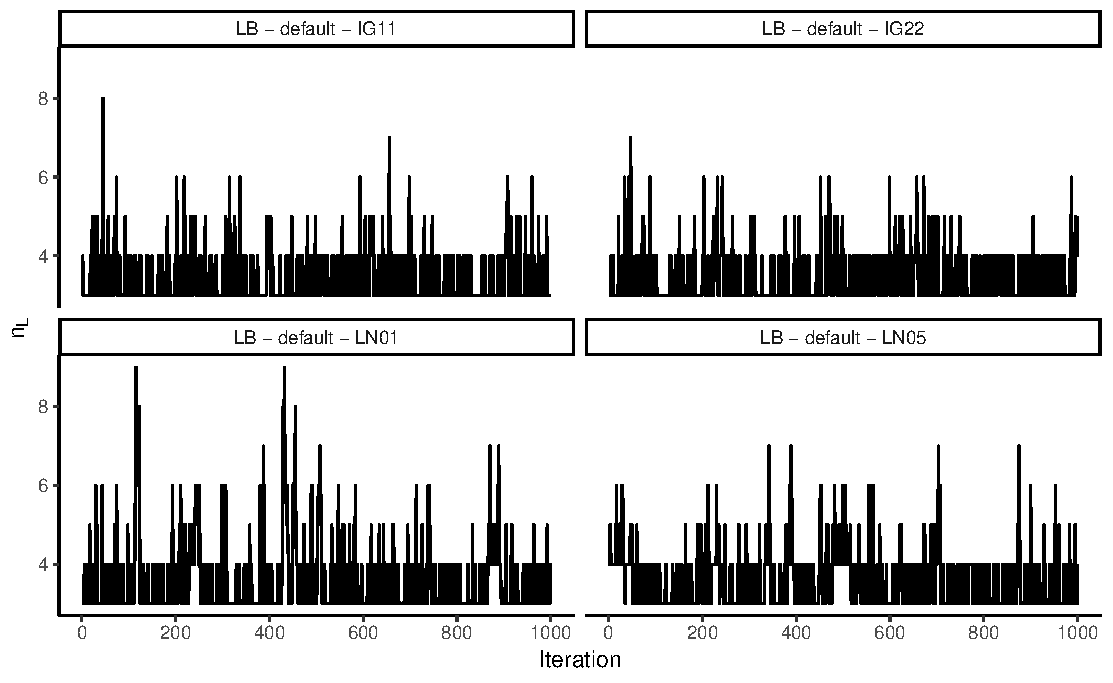
\includegraphics[width = 0.75\linewidth]{trace_case3_gumbel_nterm.pdf}
	\caption{Trace plot of $n_L$ for case 3 (\cref{eq:synth:tau_x:case3}) with Gumbel copula. The top left denotes analysis with InvInvGamma(1,1), top right denotes analysis with InvInvGamma(2,2), bottom left denotes analysis with LogNormal(0,1) and bottom right denotes analysis with LogNormal(0,5).}
	\label{fig:case3:gumbel:nterm}
\end{figure}

\begin{figure}
	\centering
	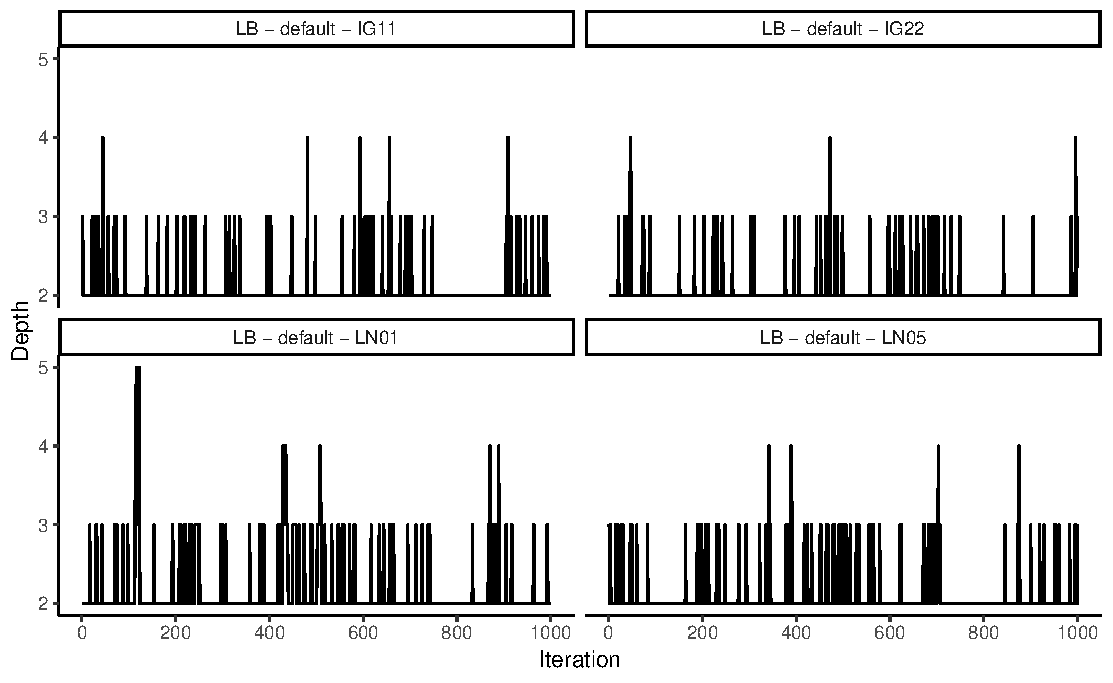
\includegraphics[width = 0.75\linewidth]{trace_case3_gumbel_depth.pdf}
	\caption{Trace plot of depth for case 3 (\cref{eq:synth:tau_x:case3}) with Gumbel copula. The top left denotes analysis with InvInvGamma(1,1), top right denotes analysis with InvInvGamma(2,2), bottom left denotes analysis with LogNormal(0,1) and bottom right denotes analysis with LogNormal(0,5).}
	\label{fig:case3:gumbel:depth}
\end{figure}

\begin{figure}
	\centering
	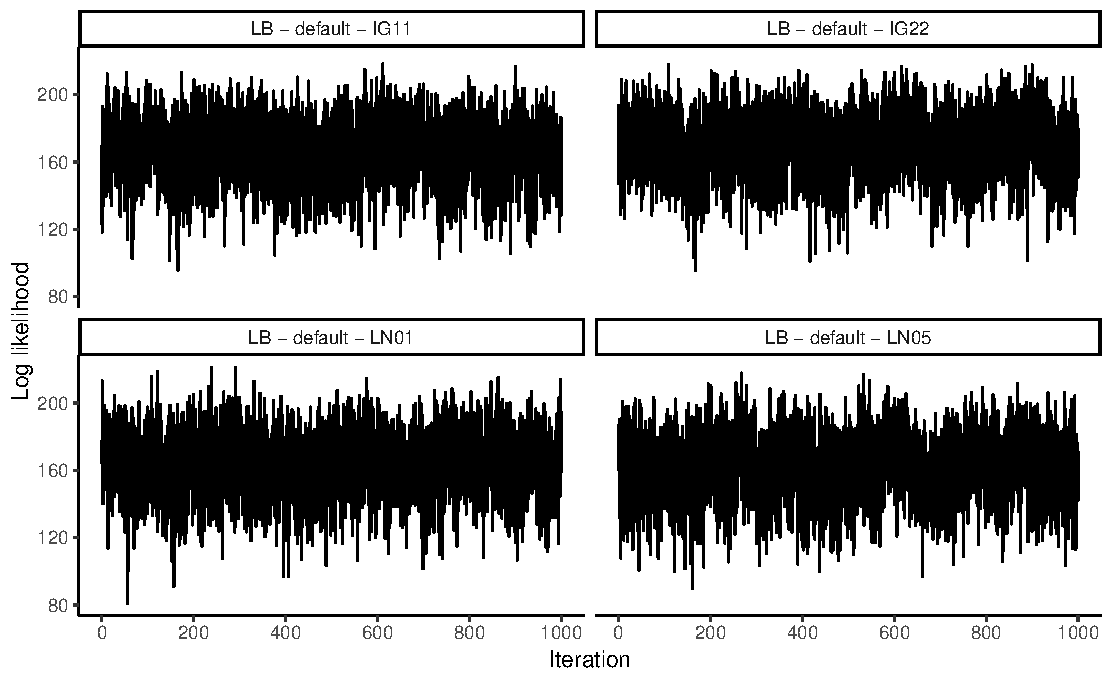
\includegraphics[width = 0.75\linewidth]{trace_case3_gumbel_like.pdf}
	\caption{Trace plot of likelihood for case 3 (\cref{eq:synth:tau_x:case3}) with Gumbel copula. The top left denotes analysis with InvInvGamma(1,1), top right denotes analysis with InvInvGamma(2,2), bottom left denotes analysis with LogNormal(0,1) and bottom right denotes analysis with LogNormal(0,5).}
	\label{fig:case3:gumbel:like}
\end{figure}

\begin{figure}
	\centering
	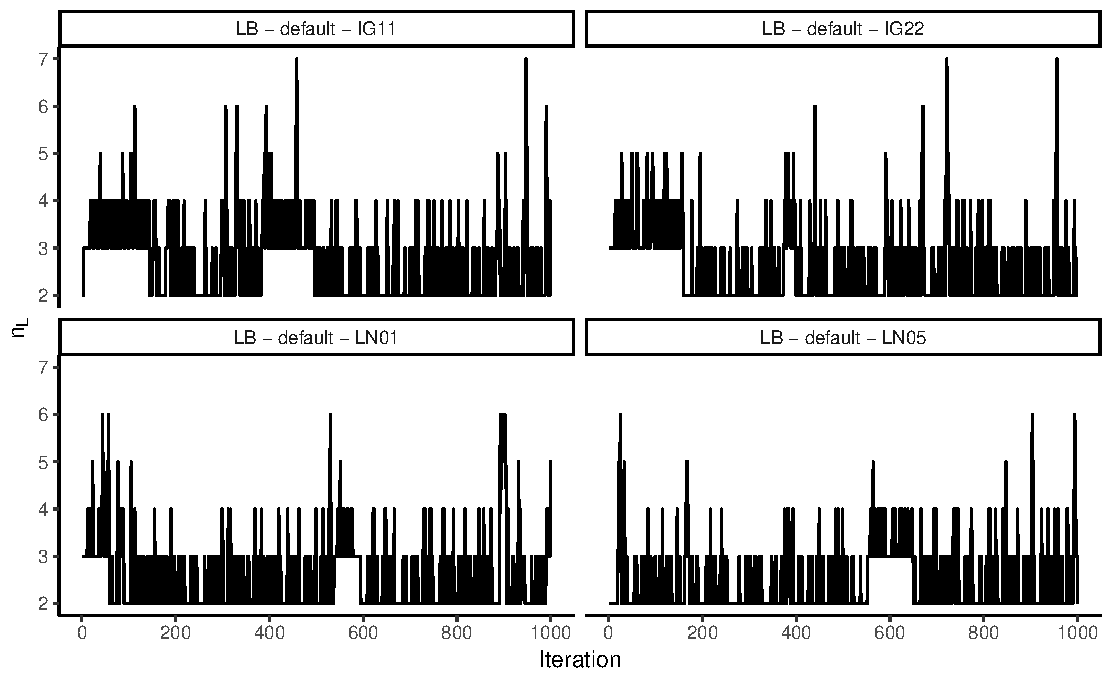
\includegraphics[width = 0.75\linewidth]{trace_case4_gumbel_nterm.pdf}
	\caption{Trace plot of $n_L$ for case 4 (\cref{eq:synth:tau_x:case4}) with Gumbel copula. The top left denotes analysis with InvInvGamma(1,1), top right denotes analysis with InvInvGamma(2,2), bottom left denotes analysis with LogNormal(0,1) and bottom right denotes analysis with LogNormal(0,5).}
	\label{fig:case4:gumbel:nterm}
\end{figure}

\begin{figure}
	\centering
	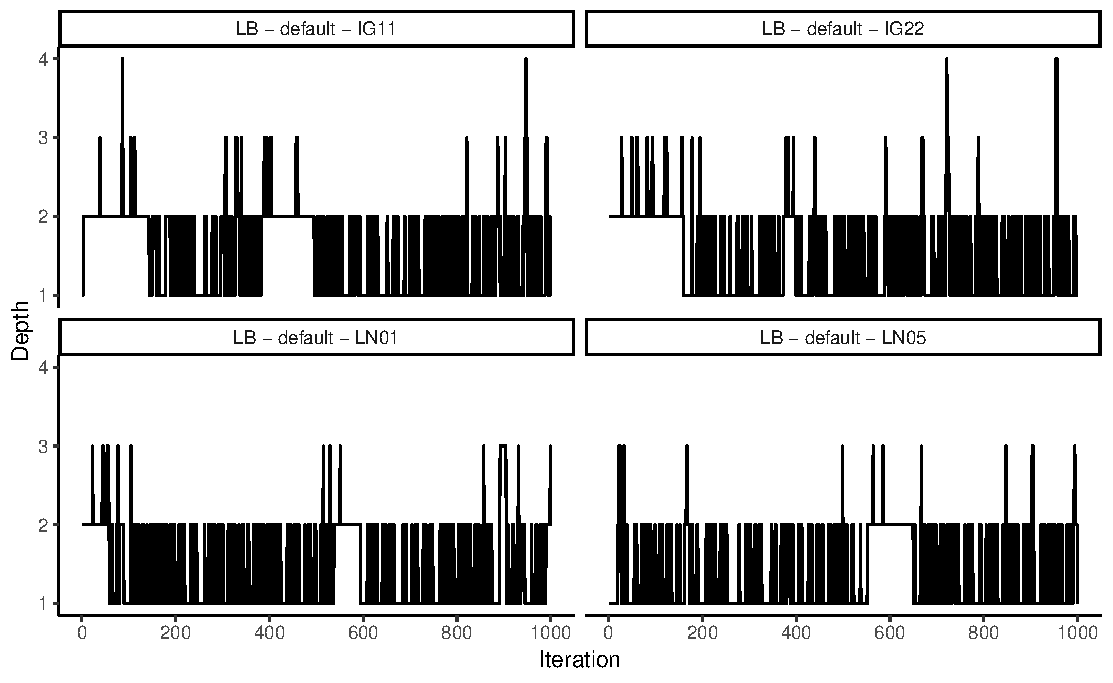
\includegraphics[width = 0.75\linewidth]{trace_case4_gumbel_depth.pdf}
	\caption{Trace plot of depth for case 4 (\cref{eq:synth:tau_x:case4}) with Gumbel copula. The top left denotes analysis with InvInvGamma(1,1), top right denotes analysis with InvInvGamma(2,2), bottom left denotes analysis with LogNormal(0,1) and bottom right denotes analysis with LogNormal(0,5).}
	\label{fig:case4:gumbel:depth}
\end{figure}

\begin{figure}
	\centering
	\includegraphics[width = 0.75\linewidth]{trace_case4_gumbel_like.pdf}
	\caption{Trace plot of likelihood for case 4 (\cref{eq:synth:tau_x:case4}) with Gumbel copula. The top left denotes analysis with InvInvGamma(1,1), top right denotes analysis with InvInvGamma(2,2), bottom left denotes analysis with LogNormal(0,1) and bottom right denotes analysis with LogNormal(0,5).}
	\label{fig:case4:gumbel:like}
\end{figure}



\bibliographystyle{plainnat}
\bibliography{example}

\end{document}
